The BulbT project was initiated at the ``Laboratoire de Machines Hydrauliques'' (LAMH) of Laval University, and aimed at investigating the flow phenomena in a bulb turbine \cite{vu2014cfd}. The turbine model consists of an intake, a bulb and a draft tube, as illustrated in Fig.~\ref{bulbt}. 
%%%%%%%%%%%%%%%%%%%%%%%%%%%%%%%%%%%%%%%%%%%%%%%%%%%%%%%%%%%
\begin{figure}[t]  
\centering
     \includegraphics[clip=true, trim= 0.0cm 0.0cm 0.0cm 0.0cm,width=0.99\linewidth]{./figures/bulbt/bulbt}                            
     \caption{Turbine model of BulbT \cite{vuillemard2014experimental}.}
     \label{bulbt}
\end{figure} 
%%%%%%%%%%%%%%%%%%%%%%%%%%%%%%%%%%%%%%%%%%%%%%%%%%%%%%%%%%%
\begin{figure}[t] 
\centering
     \includegraphics[clip=true, trim= 0.0cm 3.0cm 0.0cm 3.0cm,width=0.99\linewidth]{./figures/bulbt/bulbt-op}                  
     \caption{Operating points of BulbT \cite{vuillemard2014experimental}.}
     \label{bulbt-op}
\end{figure}
%%%%%%%%%%%%%%%%%%%%%%%%%%%%%%%%%%%%%%%%%%%%%%%%%%%%%%%%%%%
%%%%%%%%%%%%%%%%%%%%%%%%%%%%%%%%%%%%%%%%%%%%%%%%%%%%%%%%%%%

The experiments were conducted at five Operating Points (OP) as shown in Fig.~\ref{bulbt-op}. OP2 is the one closest to the best efficiency point, and the flow phenomenon is less complex compared to other OPs. Therefore, in this work, OP2 is chosen for validating the proposed schemes.
%%%%%%%%%%%%%%%%%%%%%%%%%%%%%%%%%%%%%%%%%%%%%%%%%%%%%%%%%%%
\begin{figure}[t]  
\centering
     \includegraphics[clip=true, trim= 1.75cm 6.5cm 1.75cm 0.0cm,width=0.99\linewidth]{./figures/bulbt/geometry}                            
     \caption{Geometry of the grid.}
     \label{grid}
\end{figure}
%%%%%%%%%%%%%%%%%%%%%%%%%%%%%%%%%%%%%%%%%%%%%%%%%%%%%%%%%%%

The numerical simulations were performed on three consecutively refined grids, which consist of 3M, 14M and 50M cells respectively. The grid only consists of the hub, the draft tube and an extension as shown in Fig.~\ref{grid}. No-slip boundary condition is applied to all solid walls on the rotating hub and the stationary draft tube, while slip boundary condition is imposed on the solid walls of the extension. The inlet profile is extracted from a numerical simulation conducted with the complete turbine. At the outlet, a zero pressure boundary condition is imposed. The numerical simulations were performed with the baseline MUSCL scheme, the original and extended eddy-preserving limiter scheme. The dissipation of all three schemes were scaled down with a factor of $\alpha=0.375$ in computing the convective flux,
\begin{align} 
\mathbf{F}_{i+\frac{1}{2}} =\frac{1}{2}( \mathbf{F}(\mathbf{W}_{i+\frac{1}{2}}^{L})+\mathbf{F}(\mathbf{W}_{i+\frac{1}{2}}^{R})-\alpha \mathbf{P}^{-1} \lambda (\mathbf{W}_{i+\frac{1}{2}}^{R}-\mathbf{W}_{i+\frac{1}{2}}^{L})),
\label{rusanov}
\end{align}
where $\lambda$ is the spectral radius of the preconditioned Jacobian. The numerical results computed by the three schemes are denoted by ``MUSCL'', ``EDDY'', and ``EDDY-P'' respectively.
%%%%%%%%%%%%%%%%%%%%%%%%%%%%%%%%%%%%%%%%%%%%%%%%%%%%%%%%%%%
%%%%%%%%%%%%%%%%%%%%%%%%%%%%%%%%%%%%%%%%%%%%%%%%%%%%%%%%%%%
\begin{figure}[t]  
\centering      
     \includegraphics[clip=true, trim= 0.0cm 0.0cm 0.0cm 1.0cm,width=0.99\linewidth]{./figures/bulbt/Location4B}                  
     \caption{Location of 4BY0 \cite{vuillemard2014experimental}.}
     \label{plane4BY0}
\end{figure}
%%%%%%%%%%%%%%%%%%%%%%%%%%%%%%%%%%%%%%%%%%%%%%%%%%%%%%%%%%%

In the experiment, the axial and circumferential velocity profiles were measured by the Laser Doppler Velocimetry (LDV) at 4BY0, which is the green line labeled as Axis B in Fig.~\ref{plane4BY0}. As shown in Fig.~\ref{w} and Fig.~\ref{v}, in general, the agreement against the experimental data improves as the grid is refined. On each grid, the velocity profiles computed by all schemes are almost identical. However, zoom-in views of the velocity profiles show some differences in the central region. As shown in Fig.~\ref{zw}, in the experiment, there is a backflow region in the centre of the axial velocity profile. The MUSCL scheme shows poor predictions of the backflow region on all grids, while the EDDY and EDDY-P schemes can resolve the backflow region, and the predictions improve towards the experimental data as grid was refined. As for the experimental circumferential velocity, it first accelerates from the centre point in the direction of the runner rotation gently to a local maximum, which represents a forced vortex induced by the rotating hub. It then decelerates to zero, where the flow rotational direction is reversed. The circumferential velocity then subsequently accelerates in the reversed direction to a local maximum at approximately $x=\pm 0.023$ and then decelerates, which forms a shear flow here. In Fig.~\ref{zv}, all schemes do not predict the circumferential velocity very well in the central region on the 3M grid, but on the 14M and 50M grids, the EDDY and EDDY-P schemes outperform the MUSCL scheme significantly in predicting the locations as well as the magnitudes of the local maximums. 
%%%%%%%%%%%%%%%%%%%%%%%%%%%%%%%%%%%%%%%%%%%%%%%%%%%%%%%%%%%
%%%%%%%%%%%%%%%%%%%%%%%%%%%%%%%%%%%%%%%%%%%%%%%%%%%%%%%%%%%

The results for the turbulent kinetic energy (TKE) are plotted in Fig.~\ref{tke} and Fig.~\ref{ztke}. There are two peaks in the experiment, which corresponds to the shear flows at approximately $x=\pm 0.023$. Overall, the TKE profiles were underpredicted by all schemes in most of the region. Incorrect TKE peaks appear in the central region, which are mainly due to the deviation of the computed velocity profiles. As the grid was refined, the incorrect TKE peak at the central core reduces while the two side peaks edge upwards, showing a clear improving trend towards the experimental data. On each grid, compared to the MUSCL scheme, the EDDY and EDDY-P schemes predict slightly higher values at the two side peaks and lower values in the central core region, which leads to better agreement against the experimental data. 
%%%%%%%%%%%%%%%%%%%%%%%%%%%%%%%%%%%%%%%%%%%%%%%%%%%%%%%%%%%
%%%%%%%%%%%%%%%%%%%%%%%%%%%%%%%%%%%%%%%%%%%%%%%%%%%%%%%%%%%

The pressure profiles at 4BY0 are compared in Fig.~\ref{p}. The numerical result computed by the EDDY-P scheme on the 50M grid is employed as a reference, due to the lack of an experimental distribution of pressure across the cross-section of the draft tube, and denoted by ``EDDY-P-50M''. The EDDY-P scheme was used as the reference for two reasons; first, as the grid is refined, all schemes tend towards the results of the EDDY-P scheme on the 50M grid; and second, the EDDY-P pressure distribution seems more invariant to the grid refinement. The relative $L^{2}$ norms of difference against ``EDDY-P-50M'' for all schemes on all grids are shown in Table. \ref{table2}. On the 3M grid, due to the mispredicted gradients of the circumferencial velocity near the central region, all three schemes produce incorrect peaks in the pressure profile. On the 14M grid, the incorrect peaks of EDDY and EDDY-P are almost removed, and the prediction by the MUSCL is also improved. Moreover, compared to the prediction of EDDY, the prediction of EDDY-P is closer to the reference profile EDDY-P-50M, which shows that the dissipation of the scheme is further reduced. On the 50M grid, the peak for MUSCL continues to diminish, and the predictions of EDDY and EDDY-P almost equivalent. In summary, the EDDY and EDDY-P schemes produced better pressure profiles than the MUSCL scheme, and the EDDY-P is less dissipative than EDDY as expected. 
%%%%%%%%%%%%%%%%%%%%%%%%%%%%%%%%%%%%%%%%%%%%%%%%%%%%%%%%%%%

The profiles of the vorticity magnitude at 4BY0 are plotted in Fig.~\ref{vo}. Due to lack of an experimental radial velocity profile, the experimental vorticity magnitude was computed with the assumption that the flow is uniform in the circumferential direction. Three peaks are found in the experimental profile. The central peak represents the forced vortex induced by the rotating hub, while the two side peaks represent the shear flows at approximately $x=\pm 0.023$, where the circumferential velocity accelerates to a local maximum and then decelerates. On the 3M grid, all schemes overpredict the vorticity magnitude in the centre, due to the mispredicted gradients of circumferential velocity, as shown in Fig.~\ref{v}(a). On the 14M and 50M grids, the MUSCL scheme still overpredicts the peak in the centre, while the EDDY and EDDY-P schemes only slightly underpredict the peak. It is also notable that as the grid was refined, the two side peaks due to the shear flows were captured.

%%%%%%%%%%%%%%%%%%%%%%%%%%%%%%%%%%%%%%%%%%%%%%%%%%%%%%%%%%%
The comparisons demonstrate that the original and extended eddy-preserving limiter schemes are capable of producing better predictions for velocity, TKE and pressure profiles than the baseline MUSCL scheme, and the extended eddy-preserving limiter scheme has a lower dissipation for the prediction of pressure than the original eddy-preserving limiter scheme.
%%%%%%%%%%%%%%%%%%%%%%%%%%%%%%%%%%%%%%%%%%%%%%%%%%%%%%%%%%%%%%%%
%%%%%%%%%%%%%%%%%%%%%%%%%%%%%%%%%%%%%%%%%%%%%%%%%%%%%%%%%%%%%%%%
%%%%%%%%%%%%%%%%%%%%%%%%%%%%%%%%%%%%%%%%%%%%%%%%%%%%%%%%%%%%%%%%
%%%%%%%%%%%%%%%%%%%%%%%%%%%%%%%%%%%%%%%%%%%%%%%%%%%%%%%%%%%%%%%%
%%%%%%%%%%%%%%%%%%%%%%%%%%%%%%%%%%%%%%%%%%%%%%%%%%%%%%%%%%%%%%%%
\begin{figure}[t]  
\centering
%\begin{minipage}{.99\textwidth}
\centering
     \subfigure[]{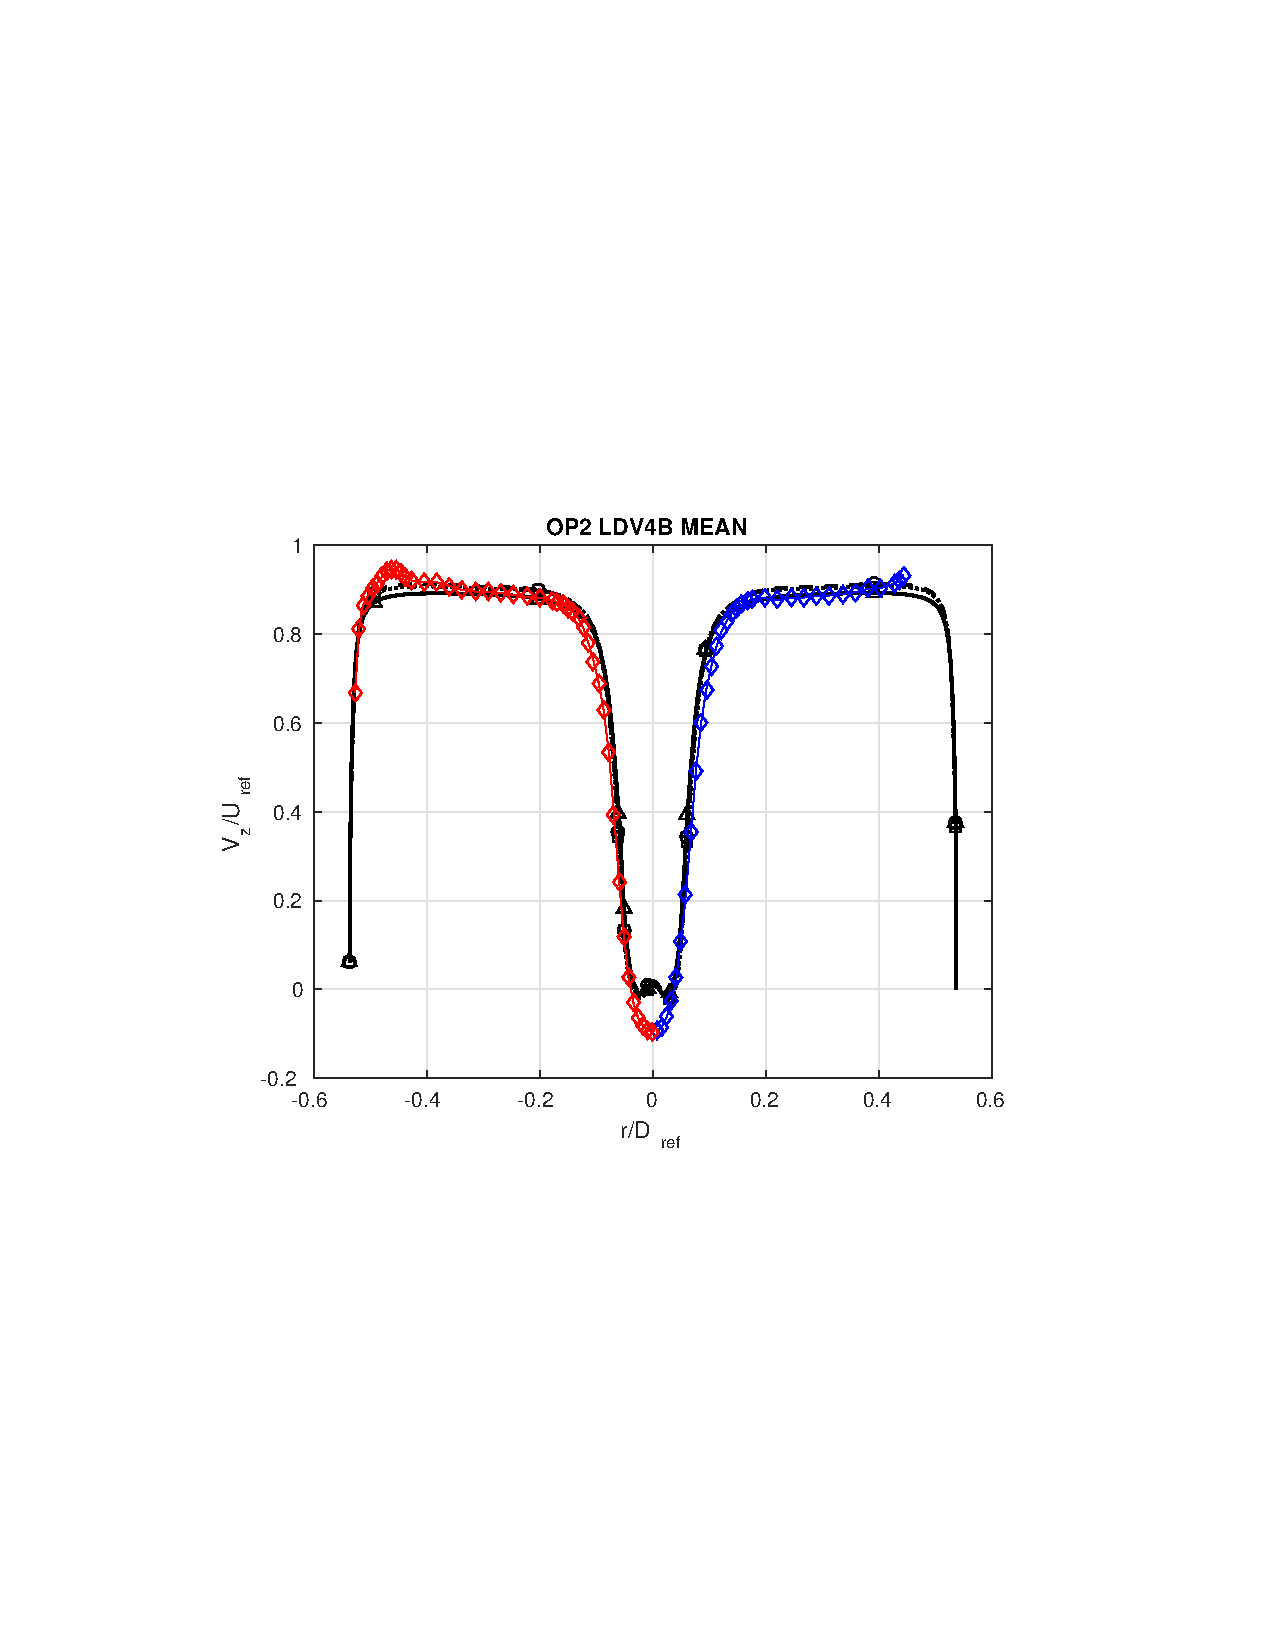
\includegraphics[clip=true, trim= 3.0cm 8.0cm 4.0cm 8.0cm,width=0.98\linewidth]{./figures/bulbt/4BY0/3m/multi_plan4BY0_BulbT_op2_uncert_X_w}} \\             
     \subfigure[]{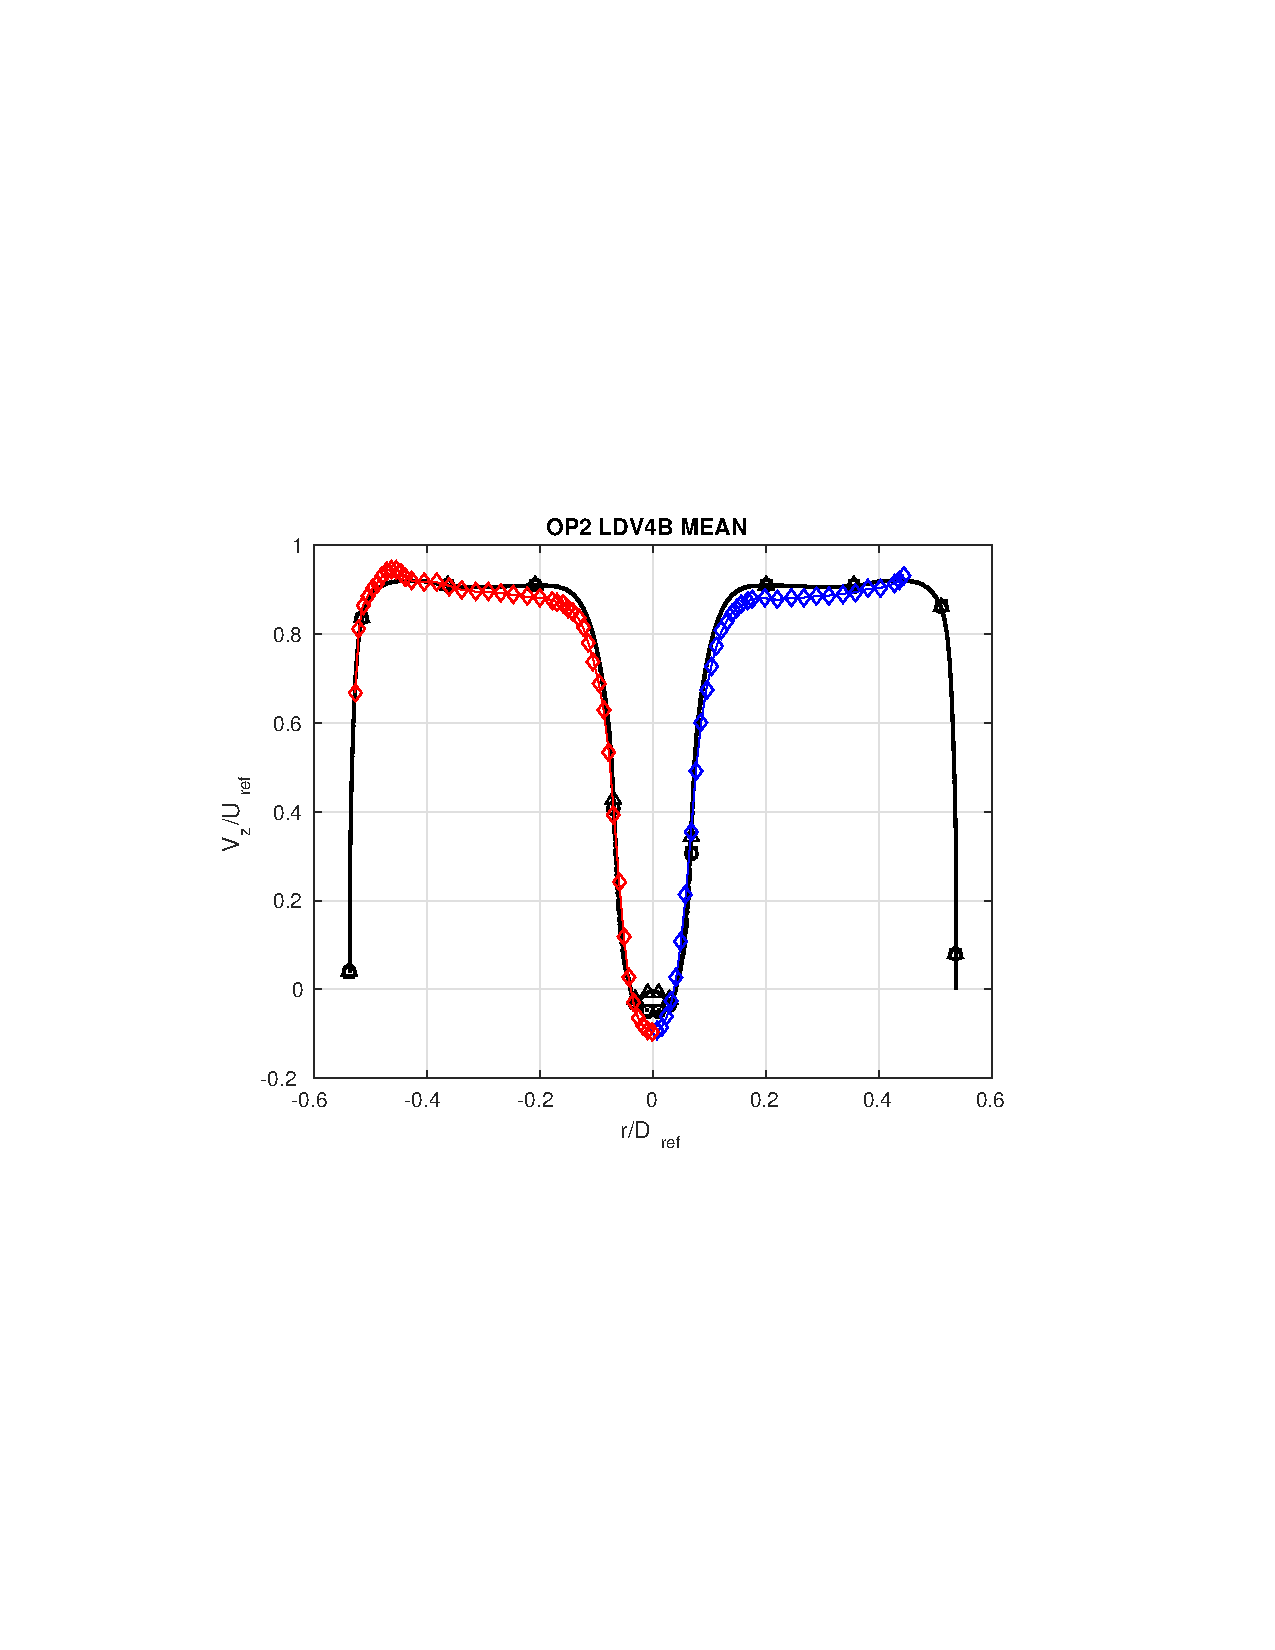
\includegraphics[clip=true, trim= 3.0cm 8.0cm 4.0cm 8.0cm,width=0.98\linewidth]{./figures/bulbt/4BY0/14m/multi_plan4BY0_BulbT_op2_uncert_X_w}} \\
     \subfigure[]{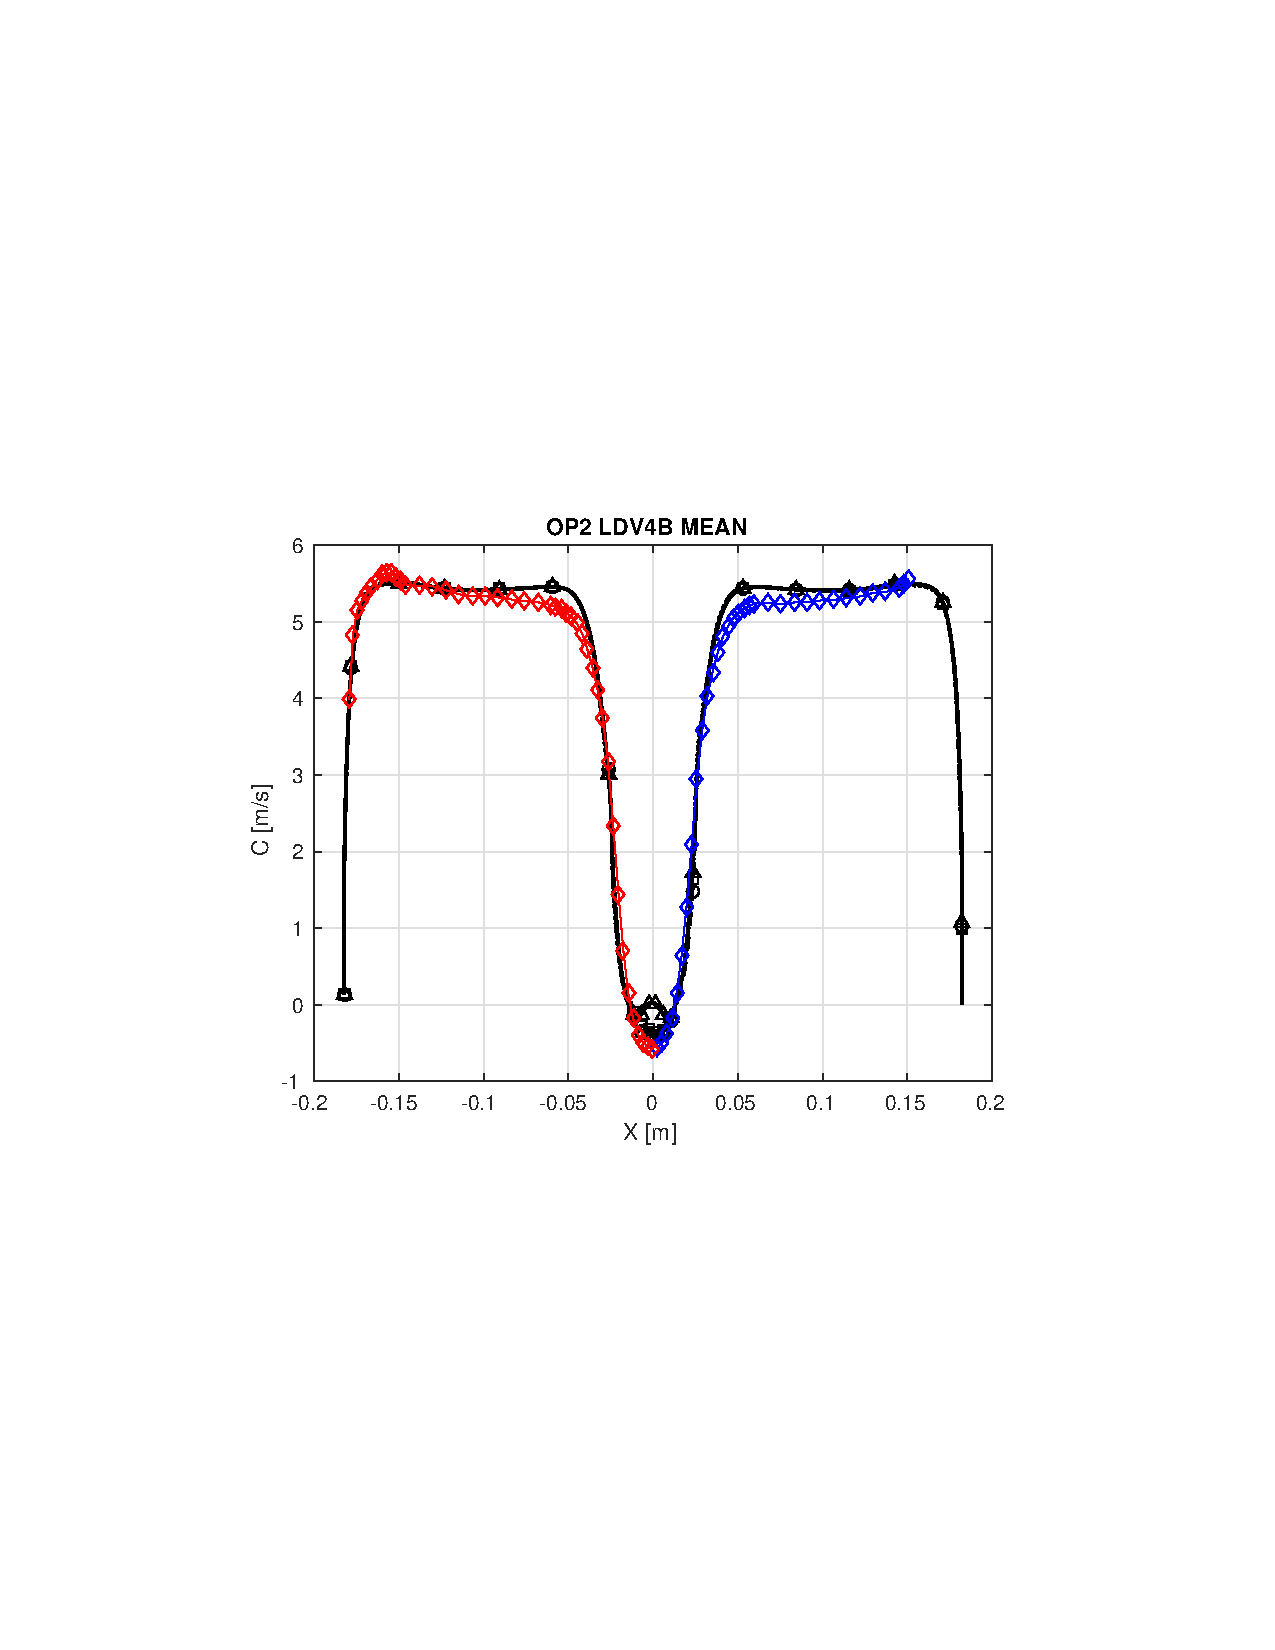
\includegraphics[clip=true, trim= 3.0cm 8.0cm 4.0cm 8.0cm,width=0.98\linewidth]{./figures/bulbt/4BY0/50m/multi_plan4BY0_BulbT_op2_uncert_X_w}}       
     \caption{Axial velocity profiles at plane 4BY0 on (a)3M (b)14M (c)50M grid. (MUSCL: \mline; EDDY: \eline; EDDY-P: \epline; EXP Cz Az0: \bluediam; EXP Cz Az180: \reddiam.)}
     \label{w} 
%     \end{minipage}          
\end{figure}
%%%%%%%%%%%%%%%%%%%%%%%%%%%%%%%%%%%%%%%%%%%%%%%%%%%%%%%%%%%%%%%%
\begin{figure}[t]  
\centering
%\begin{minipage}{.99\textwidth}
\centering
     \subfigure[]{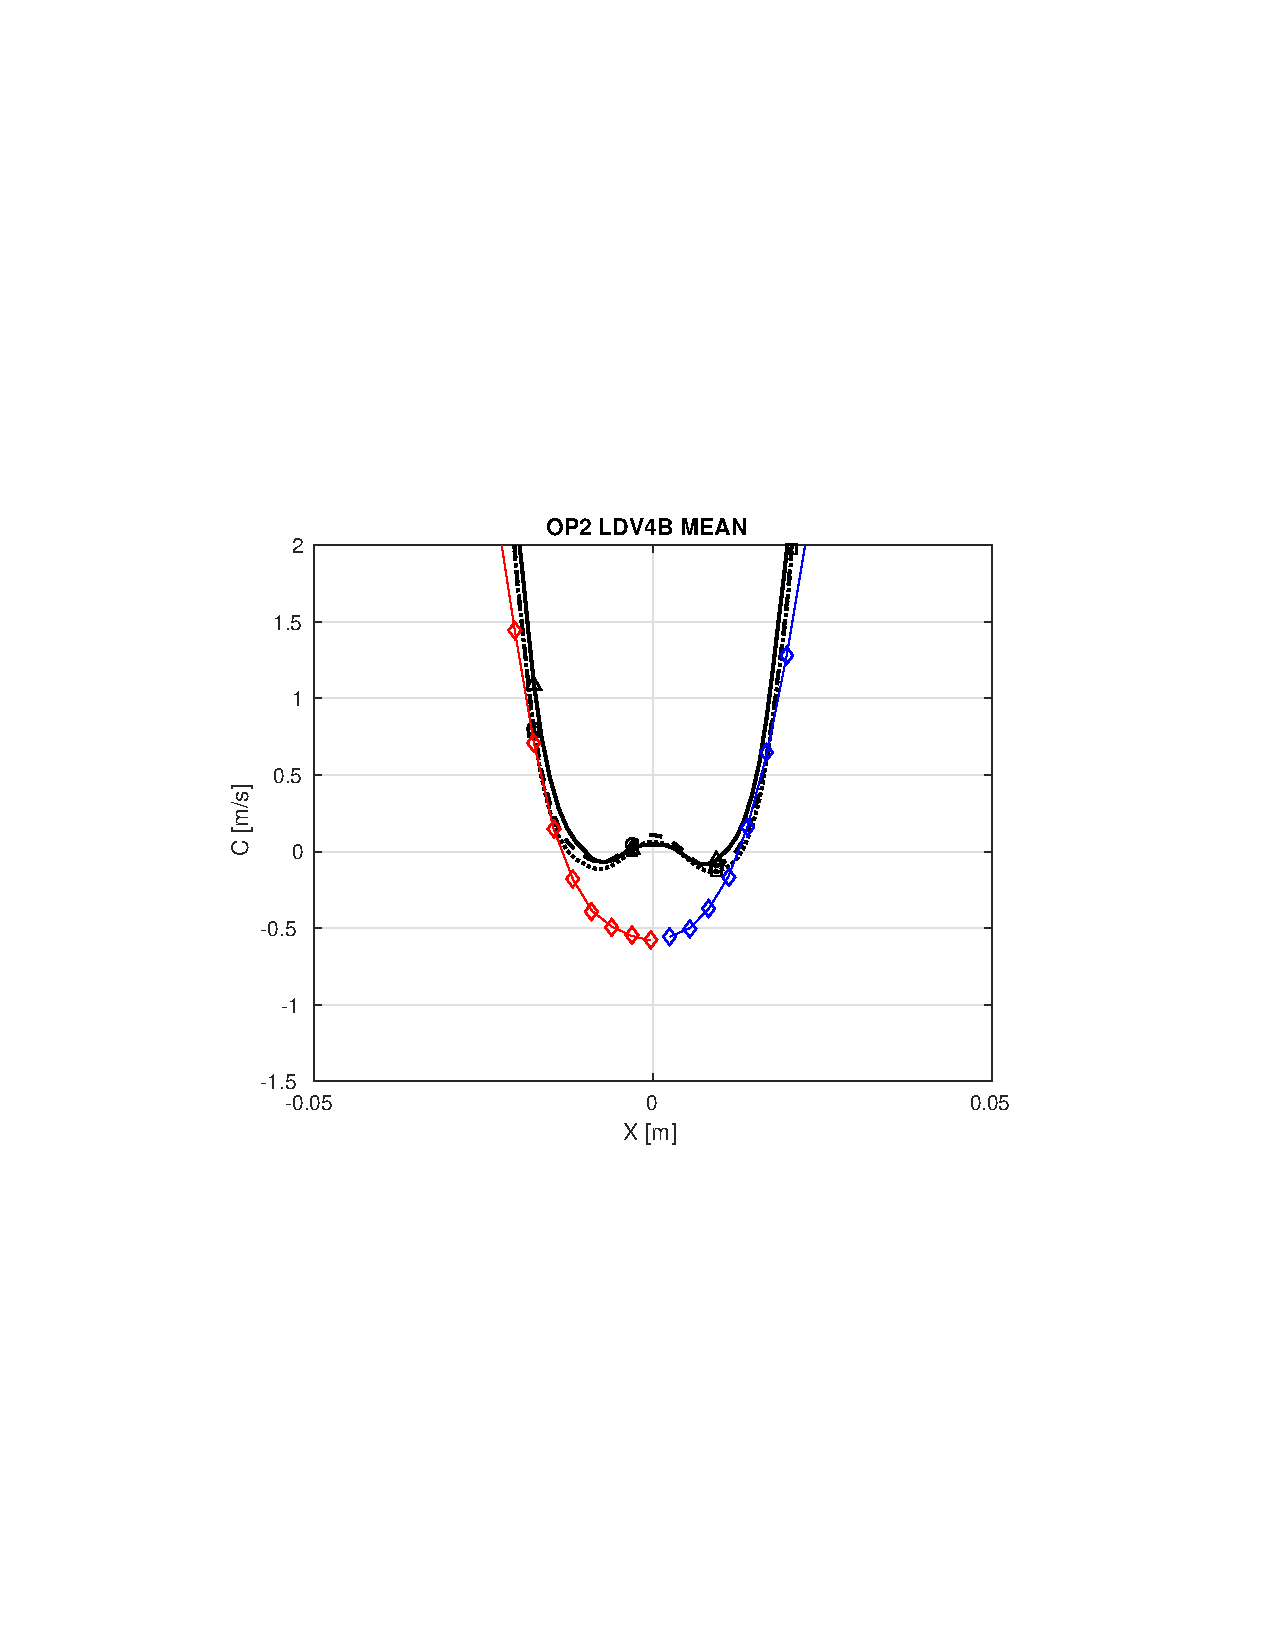
\includegraphics[clip=true, trim= 3.0cm 8.0cm 4.0cm 8.0cm,width=0.98\linewidth]{./figures/bulbt/4BY0/3m/zoom_multi_plan4BY0_BulbT_op2_uncert_X_w}} \\             
     \subfigure[]{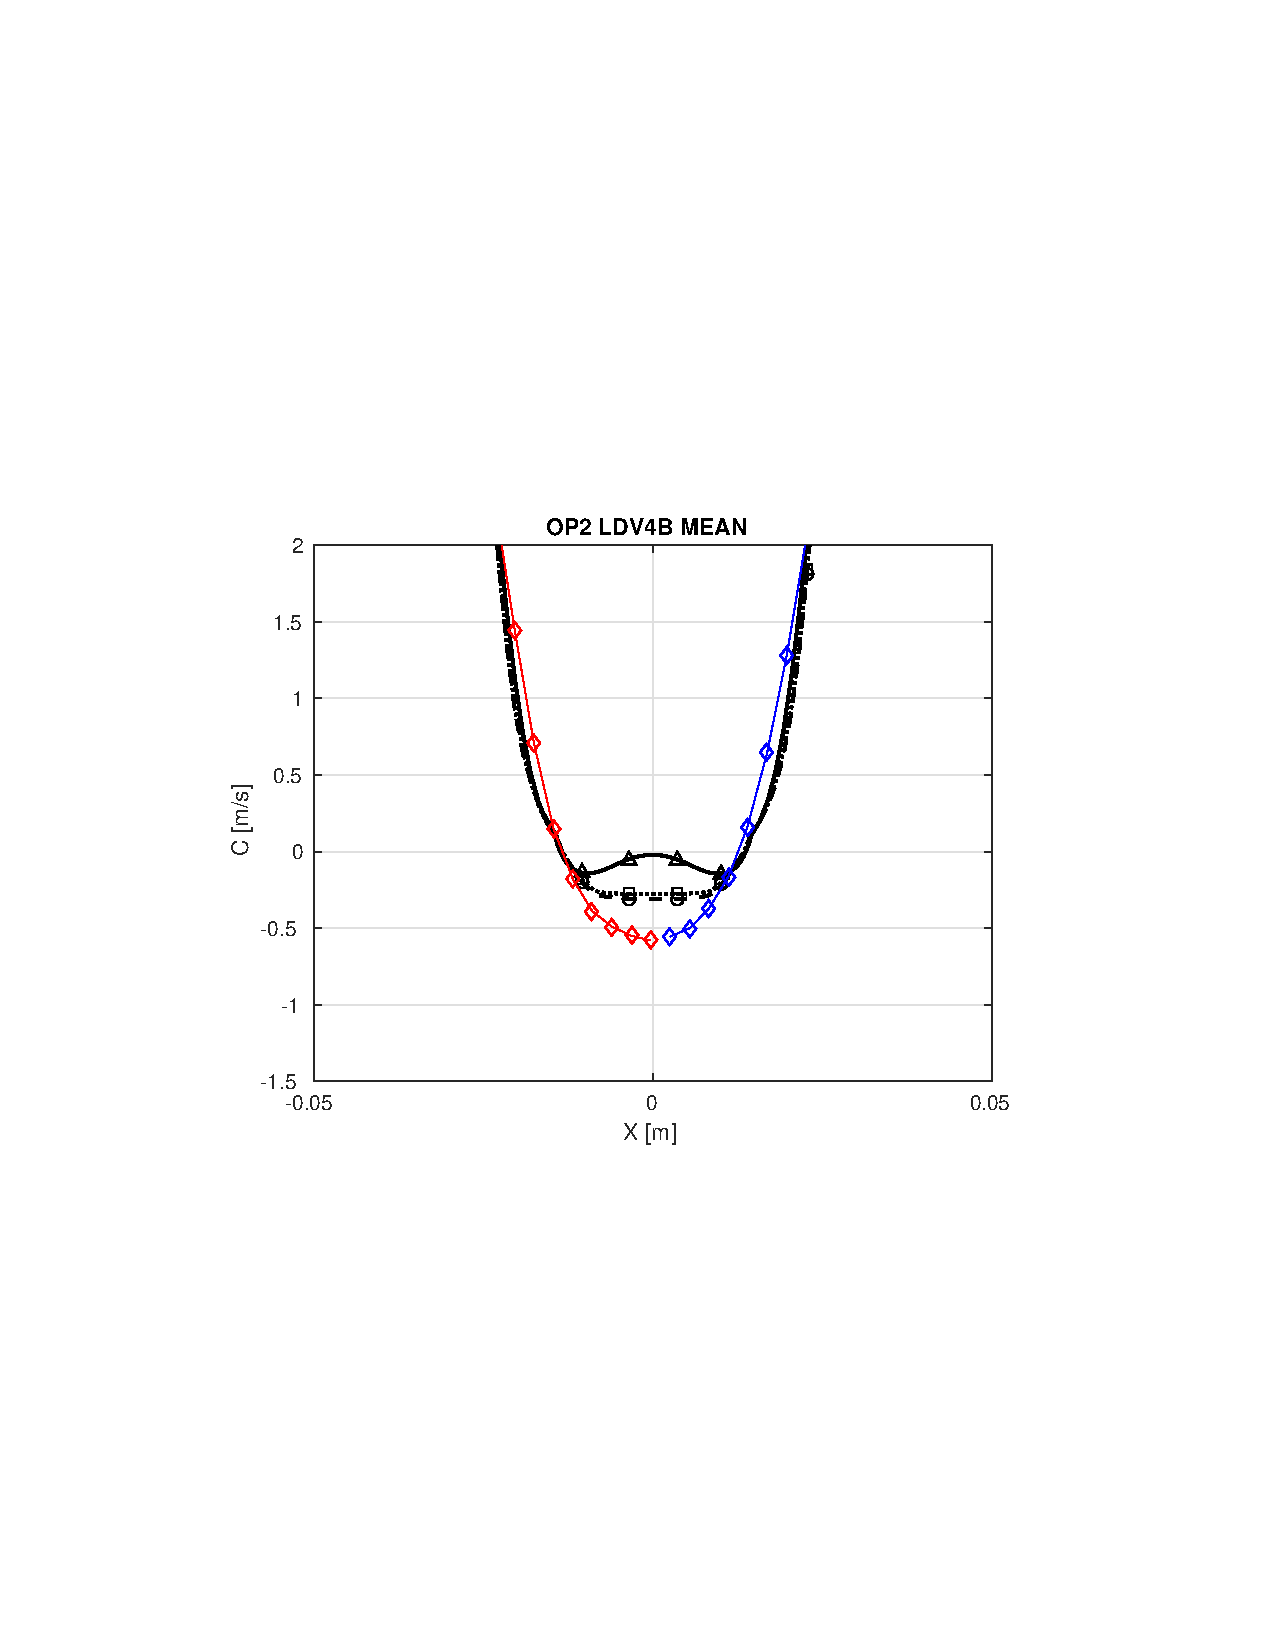
\includegraphics[clip=true, trim= 3.0cm 8.0cm 4.0cm 8.0cm,width=0.98\linewidth]{./figures/bulbt/4BY0/14m/zoom_multi_plan4BY0_BulbT_op2_uncert_X_w}} \\
     \subfigure[]{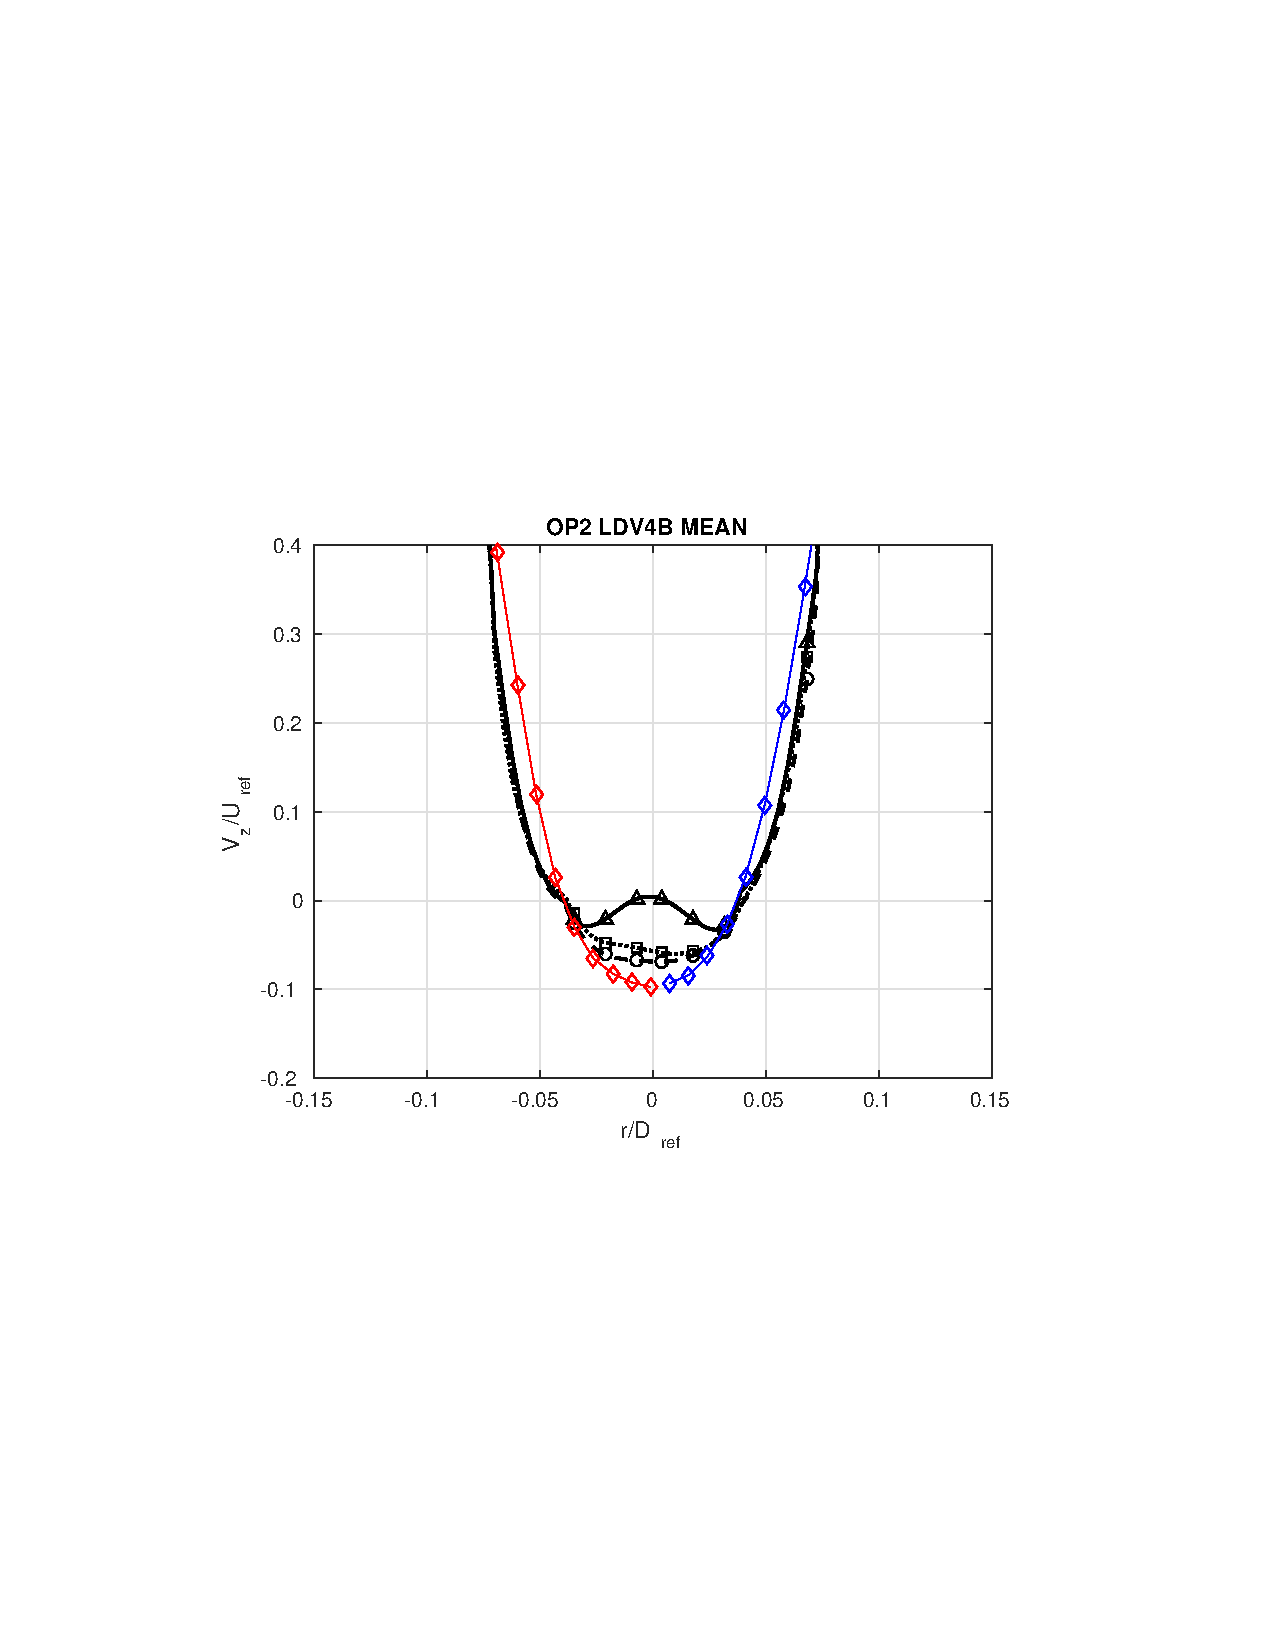
\includegraphics[clip=true, trim= 3.0cm 8.0cm 4.0cm 8.0cm,width=0.98\linewidth]{./figures/bulbt/4BY0/50m/zoom_multi_plan4BY0_BulbT_op2_uncert_X_w}}     
     \caption{Zoom-in view of axial velocity profiles at plane 4BY0 on (a)3M (b)14M (c)50M grid. (MUSCL: \mline; EDDY: \eline; EDDY-P: \epline; EXP Cz Az0: \bluediam; EXP Cz Az180: \reddiam.)}
     \label{zw} 
%     \end{minipage}          
\end{figure}
%%%%%%%%%%%%%%%%%%%%%%%%%%%%%%%%%%%%%%%%%%%%%%%%%%%%%%%%%%%%%%%%
%%%%%%%%%%%%%%%%%%%%%%%%%%%%%%%%%%%%%%%%%%%%%%%%%%%%%%%%%%%%%%%%
\begin{figure}[t]  
\centering
%\begin{minipage}{.99\textwidth}
\centering
     \subfigure[]{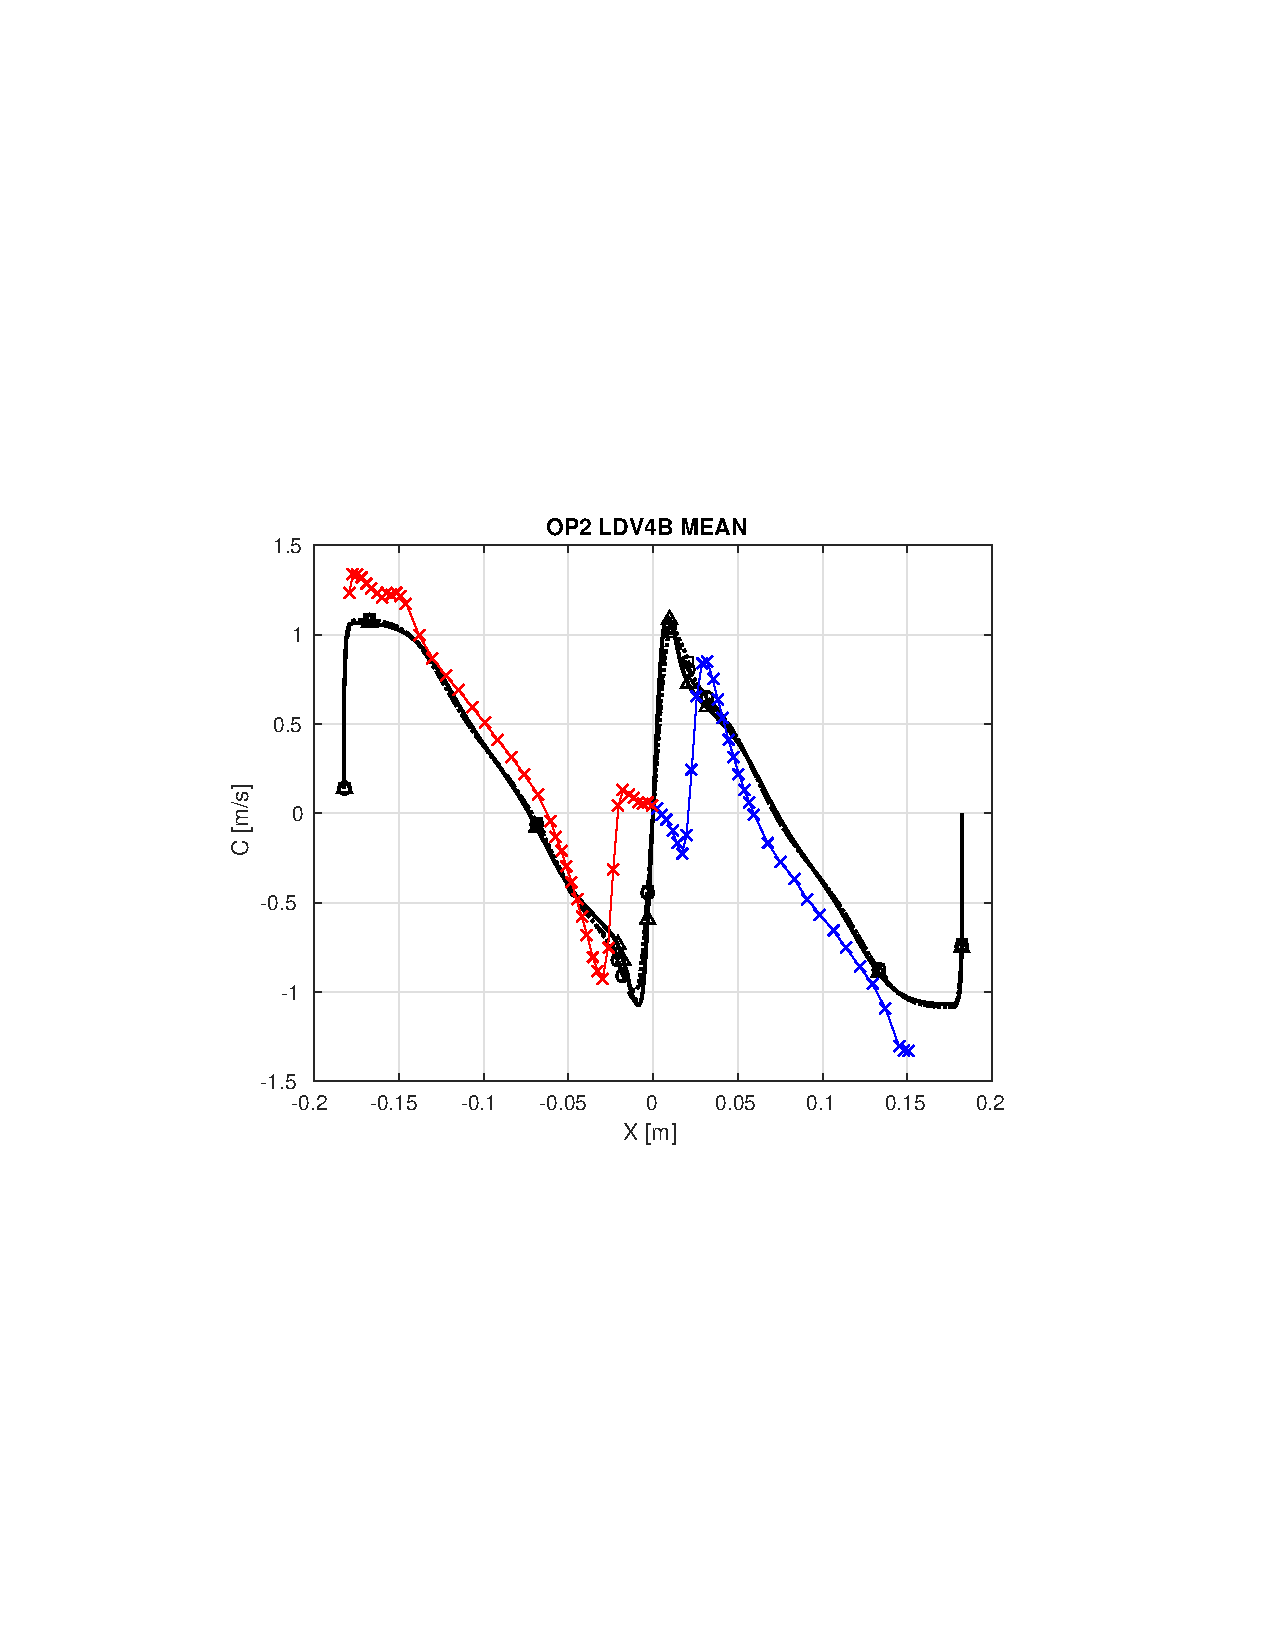
\includegraphics[clip=true, trim= 3.0cm 8.0cm 4.0cm 8.0cm,width=0.98\linewidth]{./figures/bulbt/4BY0/3m/multi_plan4BY0_BulbT_op2_uncert_X_v}} \\             
     \subfigure[]{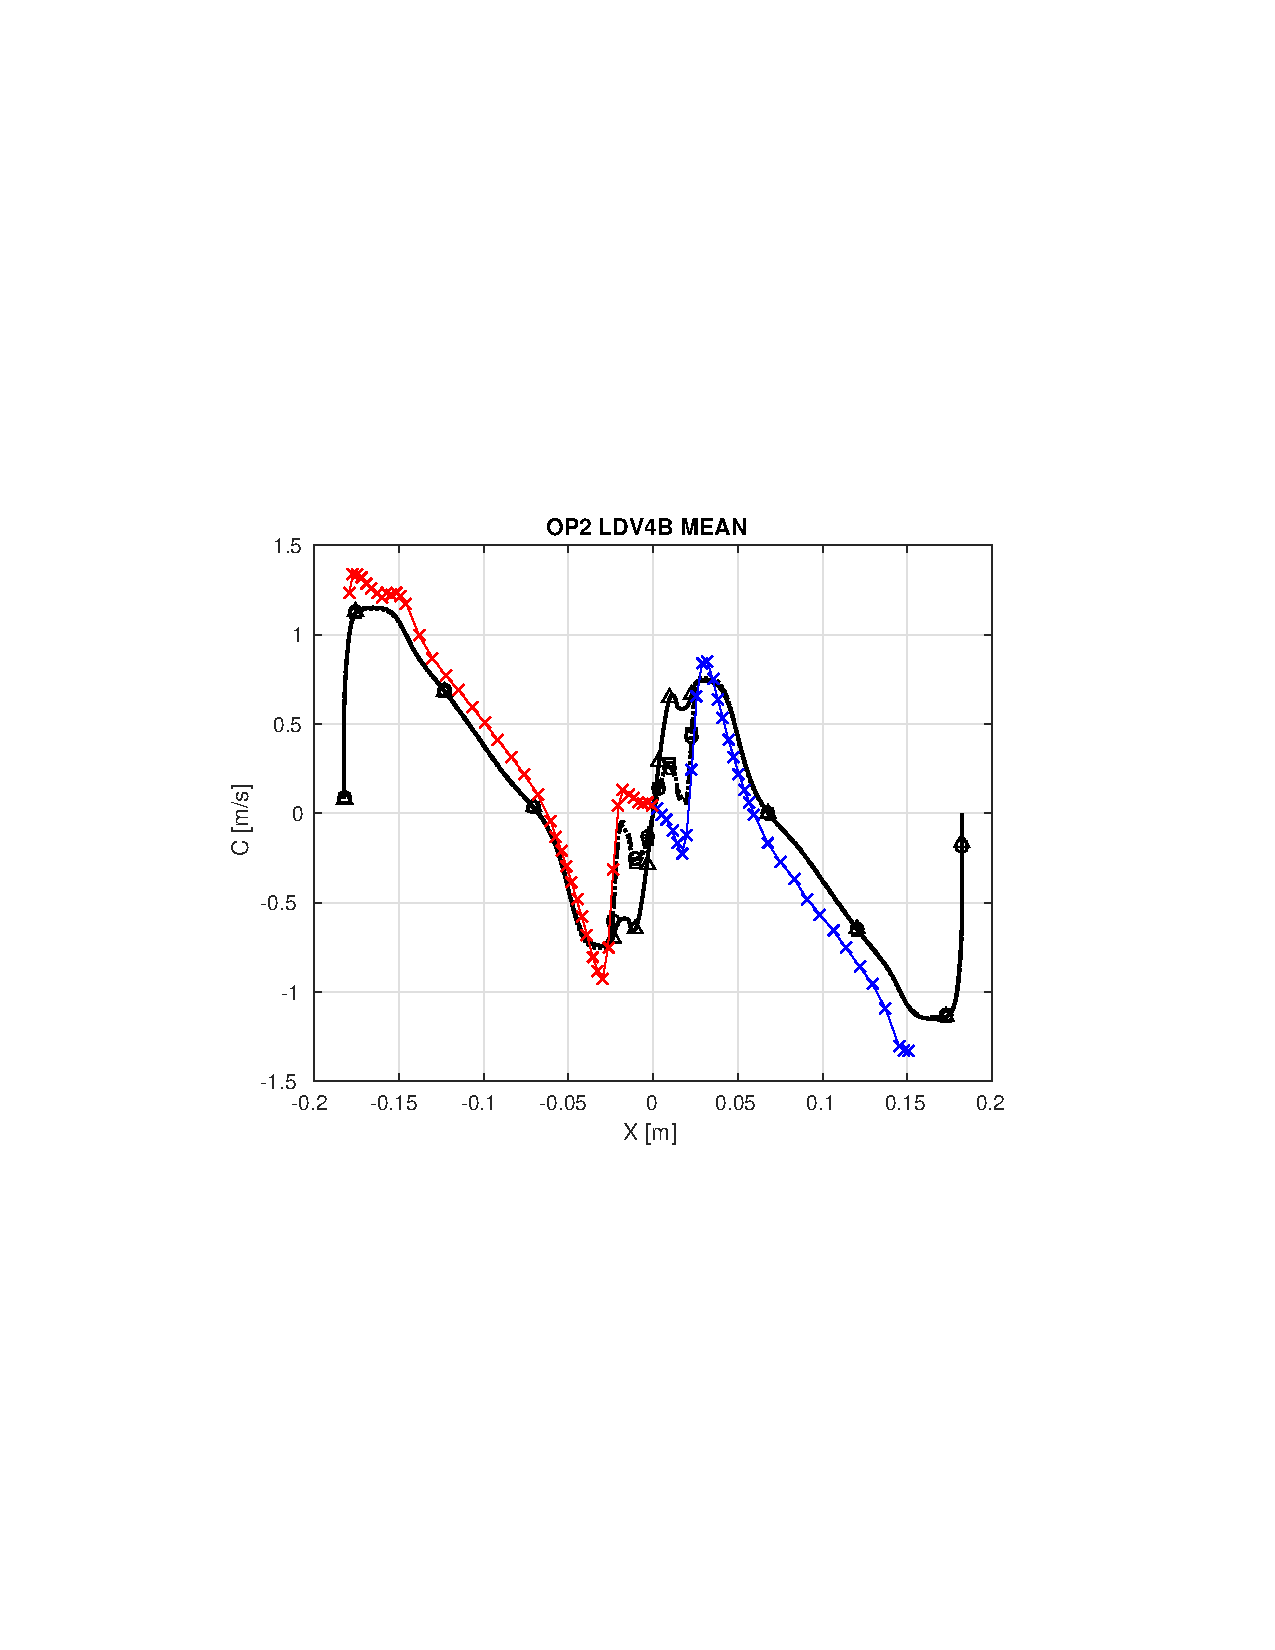
\includegraphics[clip=true, trim= 3.0cm 8.0cm 4.0cm 8.0cm,width=0.98\linewidth]{./figures/bulbt/4BY0/14m/multi_plan4BY0_BulbT_op2_uncert_X_v}} \\
     \subfigure[]{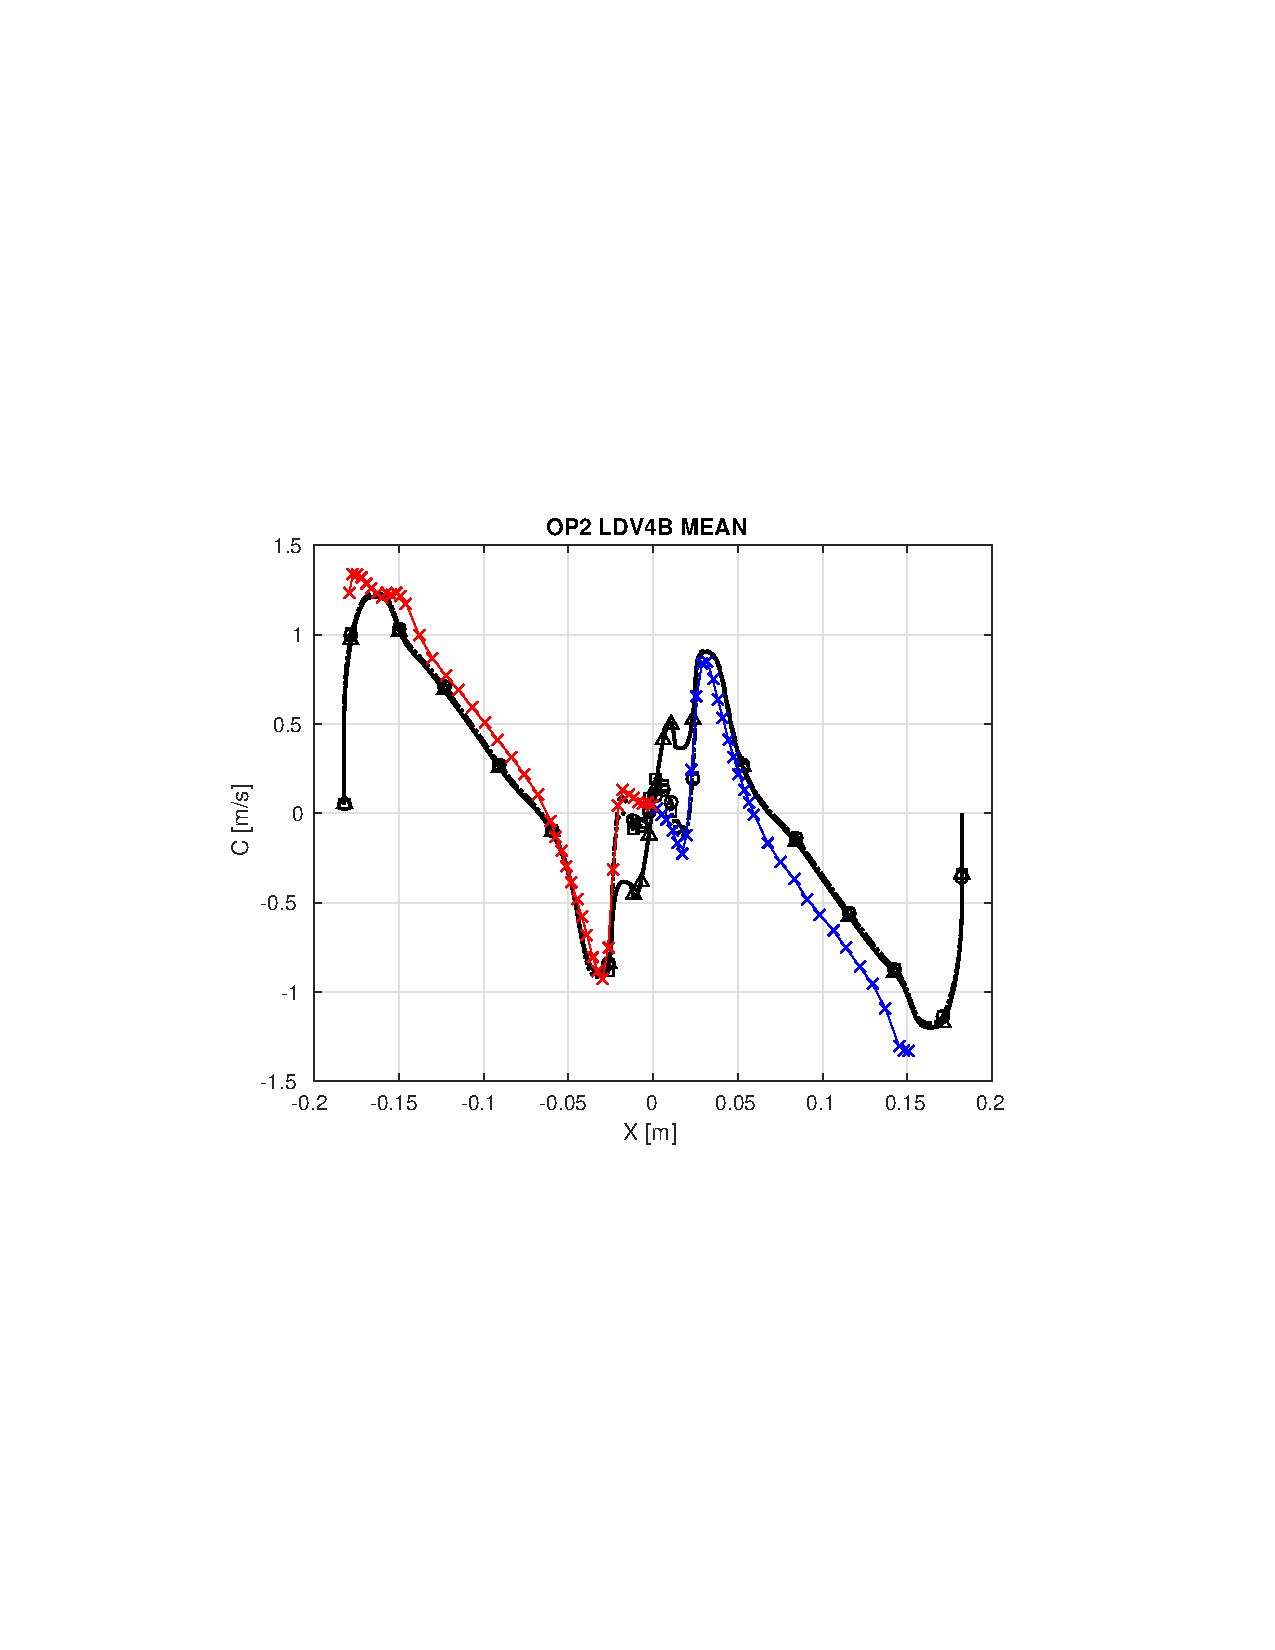
\includegraphics[clip=true, trim= 3.0cm 8.0cm 4.0cm 8.0cm,width=0.98\linewidth]{./figures/bulbt/4BY0/50m/multi_plan4BY0_BulbT_op2_uncert_X_v}}     
     \caption{Circumferential velocity profiles at plane 4BY0 on (a)3M (b)14M (c)50M grid. (MUSCL: \mline; EDDY: \eline; EDDY-P: \epline; EXP Cy Az0: \bluecrx; EXP Cy Az180: \redcrx.)}
     \label{v} 
%     \end{minipage}          
\end{figure}
%%%%%%%%%%%%%%%%%%%%%%%%%%%%%%%%%%%%%%%%%%%%%%%%%%%%%%%%%%%%%%%%
\begin{figure}[t]  
\centering
%\begin{minipage}{.99\textwidth}
\centering
     \subfigure[]{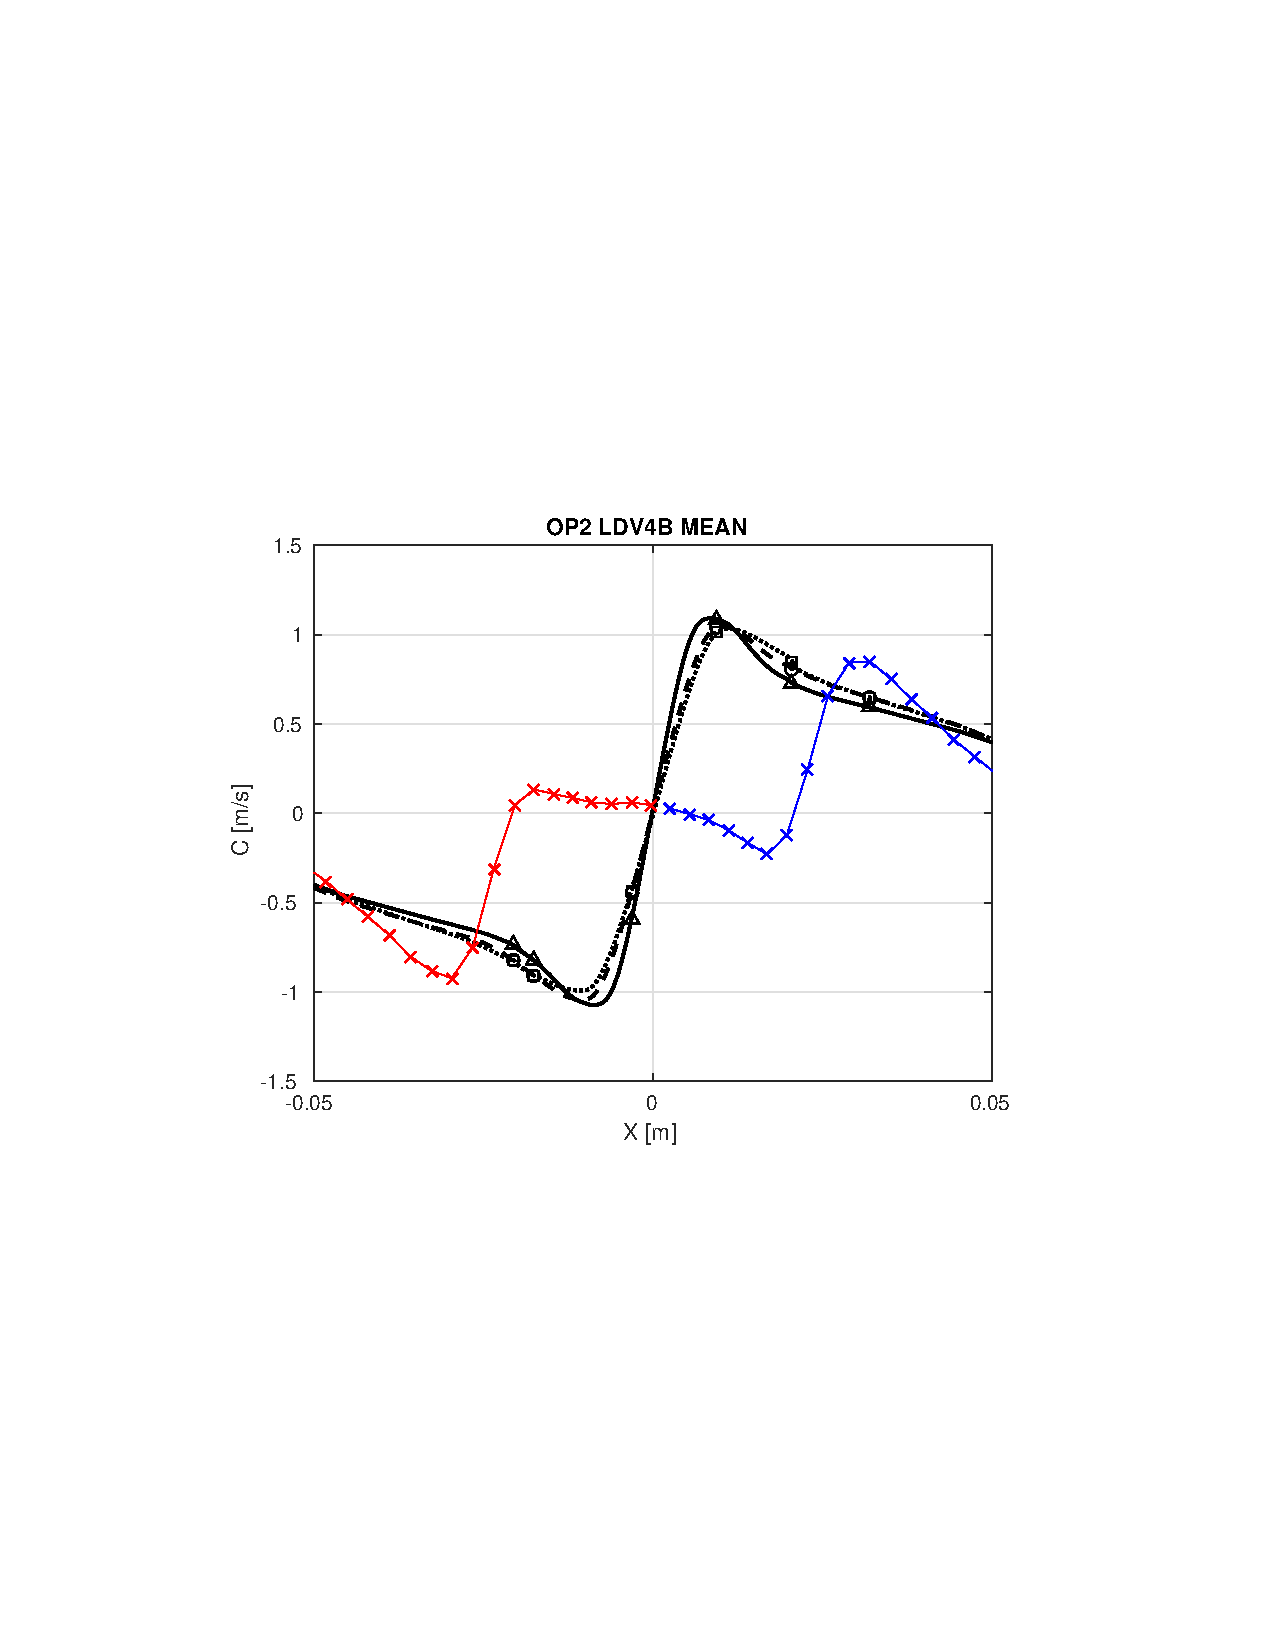
\includegraphics[clip=true, trim= 3.0cm 8.0cm 4.0cm 8.0cm,width=0.98\linewidth]{./figures/bulbt/4BY0/3m/zoom_multi_plan4BY0_BulbT_op2_uncert_X_v}} \\             
     \subfigure[]{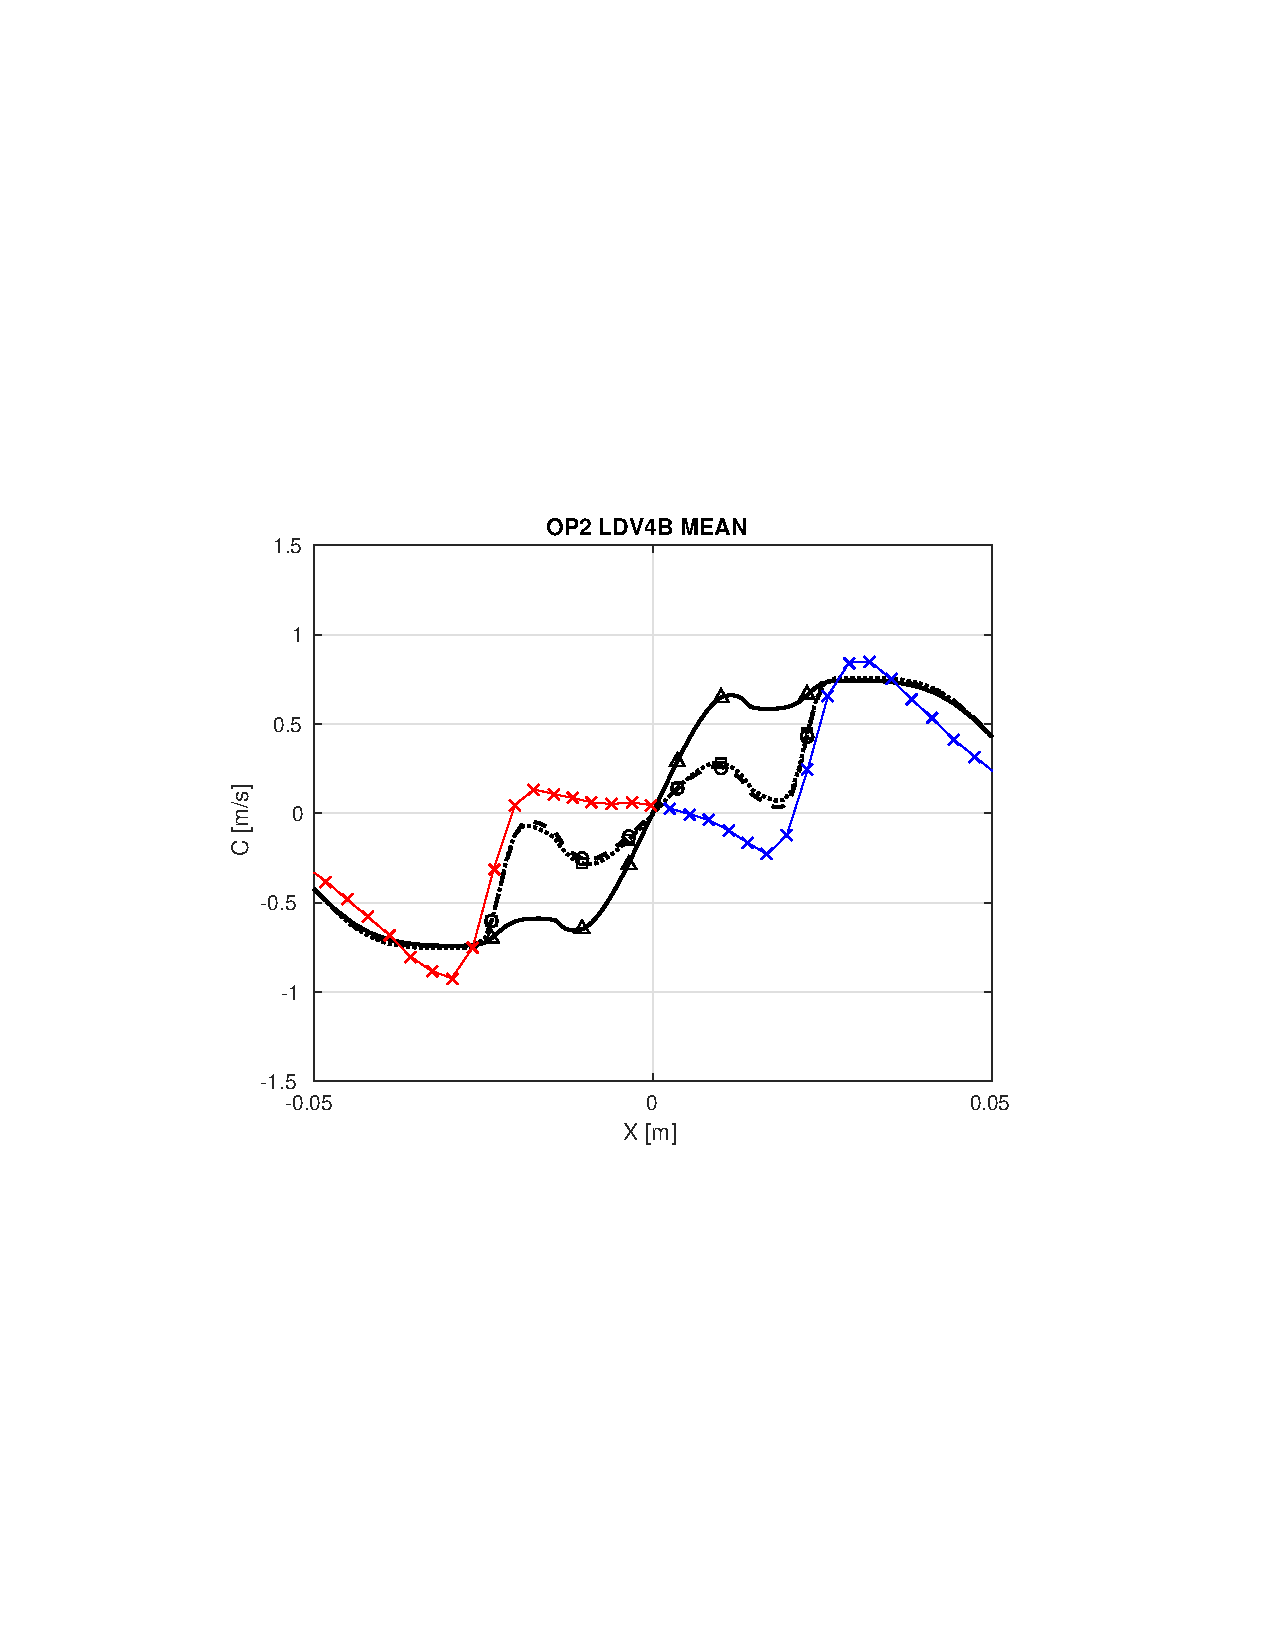
\includegraphics[clip=true, trim= 3.0cm 8.0cm 4.0cm 8.0cm,width=0.98\linewidth]{./figures/bulbt/4BY0/14m/zoom_multi_plan4BY0_BulbT_op2_uncert_X_v}} \\
     \subfigure[]{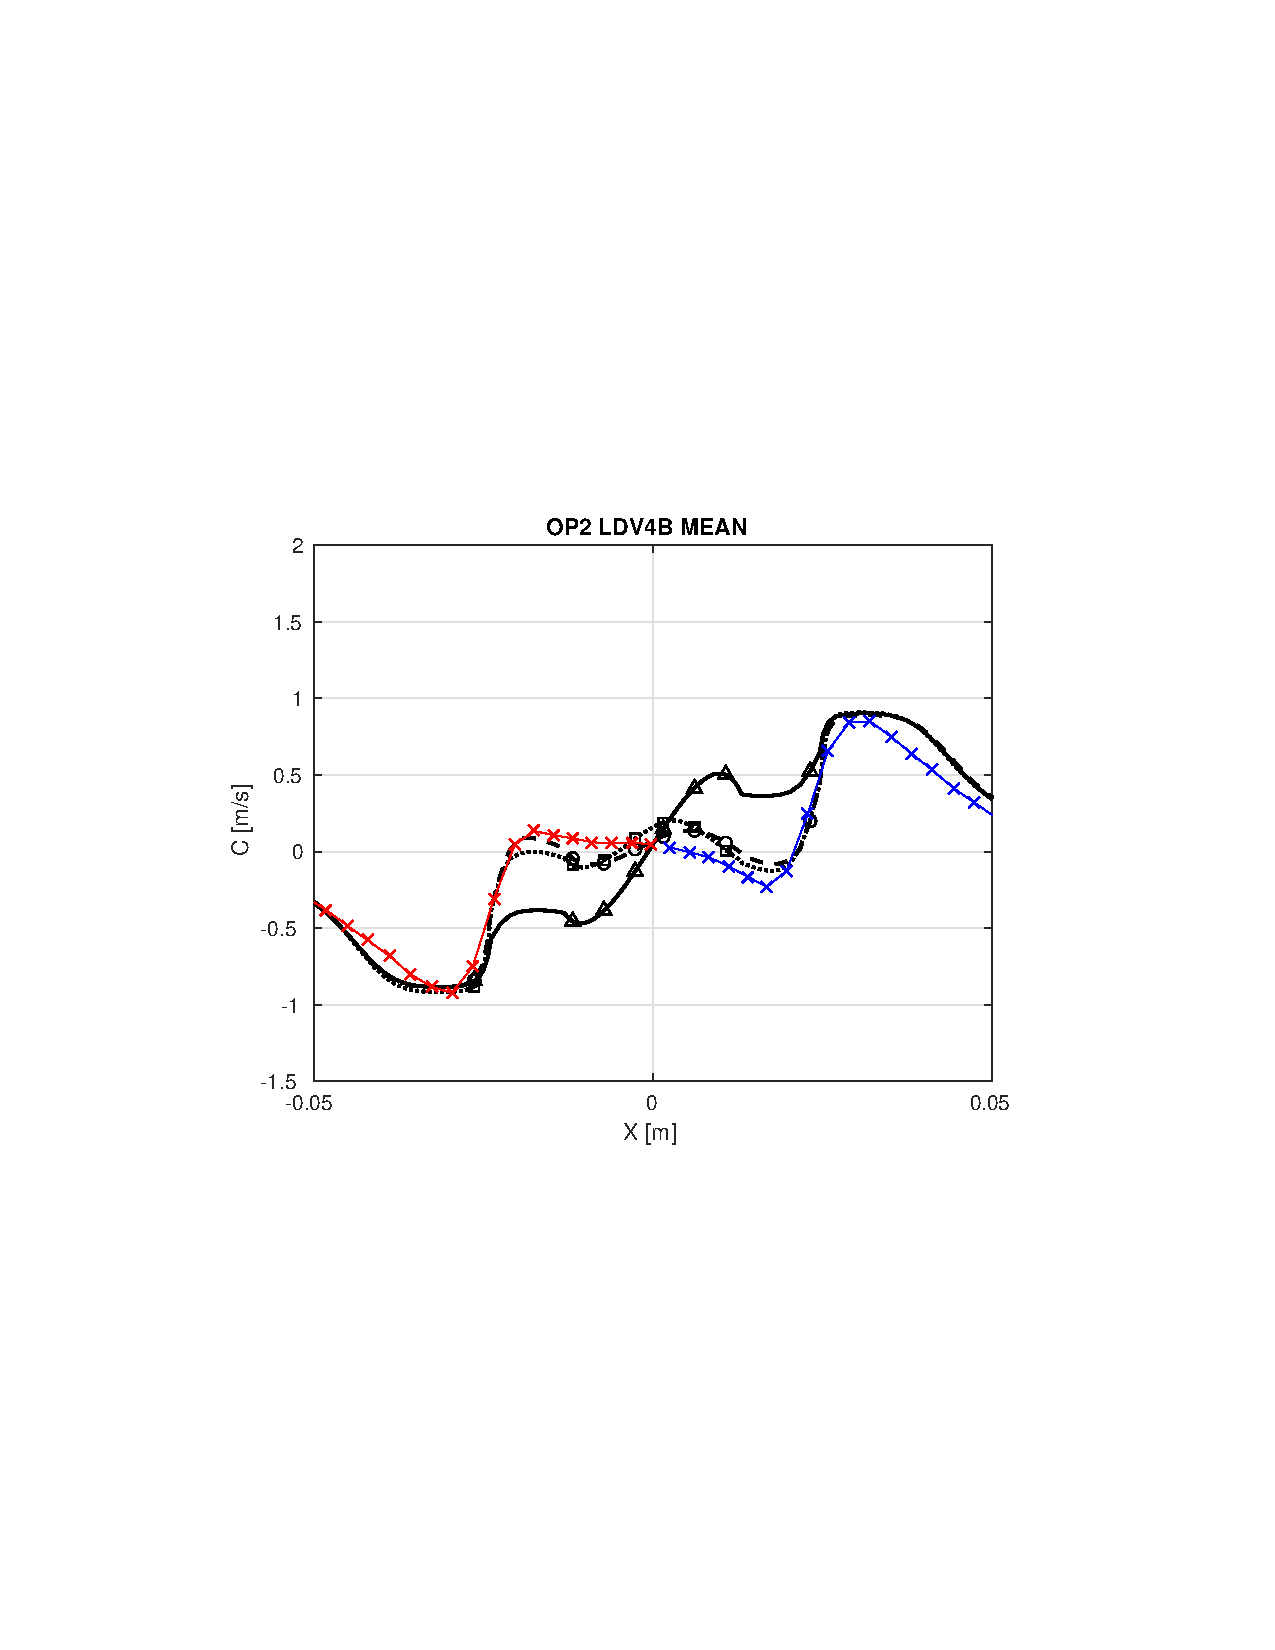
\includegraphics[clip=true, trim= 3.0cm 8.0cm 4.0cm 8.0cm,width=0.98\linewidth]{./figures/bulbt/4BY0/50m/zoom_multi_plan4BY0_BulbT_op2_uncert_X_v}}        
     \caption{Zoom-in view of circumferential velocity profiles at plane 4BY0 on (a)3M (b)14M (c)50M grid. (MUSCL: \mline; EDDY: \eline; EDDY-P: \epline; EXP Cy Az0: \bluecrx; EXP Cy Az180: \redcrx.)}
     \label{zv} 
%     \end{minipage}          
\end{figure}
%%%%%%%%%%%%%%%%%%%%%%%%%%%%%%%%%%%%%%%%%%%%%%%%%%%%%%%%%%%%%%%%
%%%%%%%%%%%%%%%%%%%%%%%%%%%%%%%%%%%%%%%%%%%%%%%%%%%%%%%%%%%%%%%%
\begin{figure}[t]  
\centering
%\begin{minipage}{.99\textwidth}
\centering
     \subfigure[]{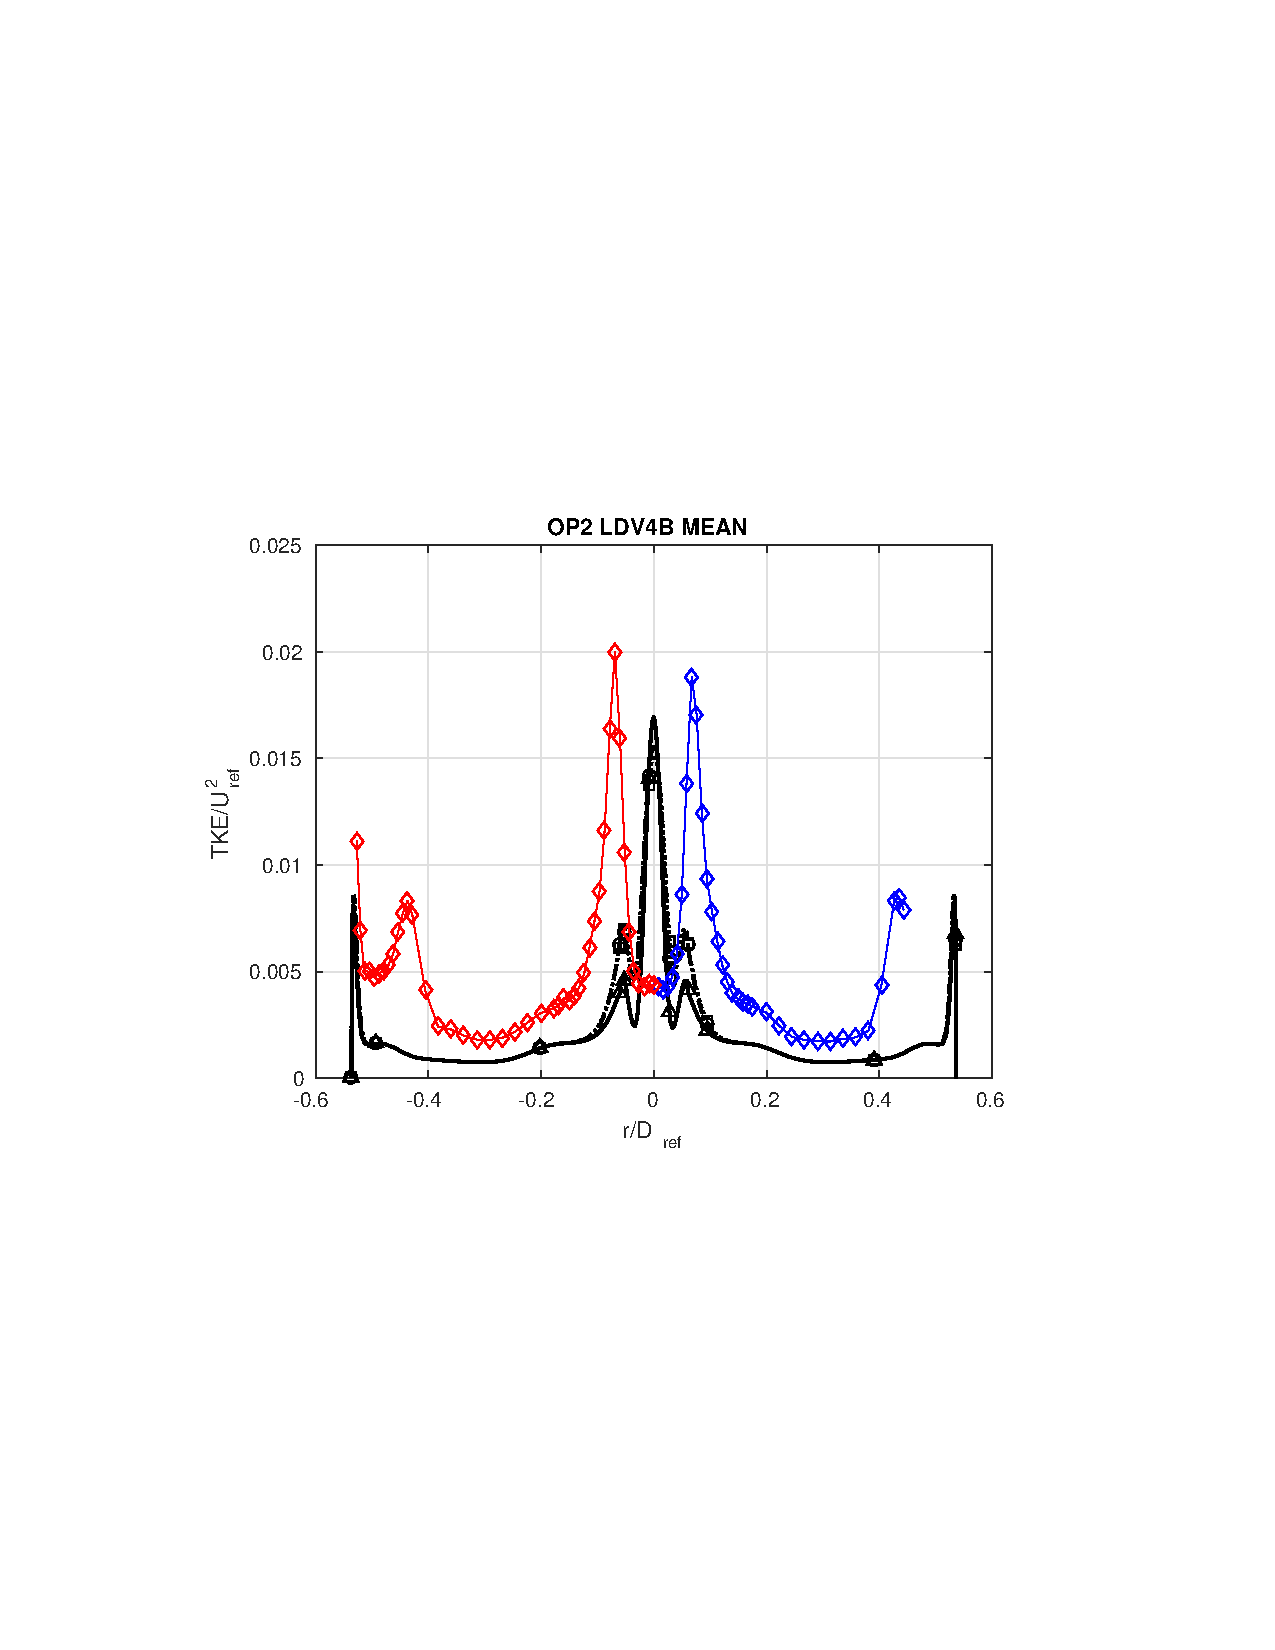
\includegraphics[clip=true, trim= 3.0cm 8.0cm 4.0cm 8.0cm,width=0.98\linewidth]{./figures/bulbt/4BY0/3m/multi_plan4BY0_BulbT_op2_Tke_X}} \\             
     \subfigure[]{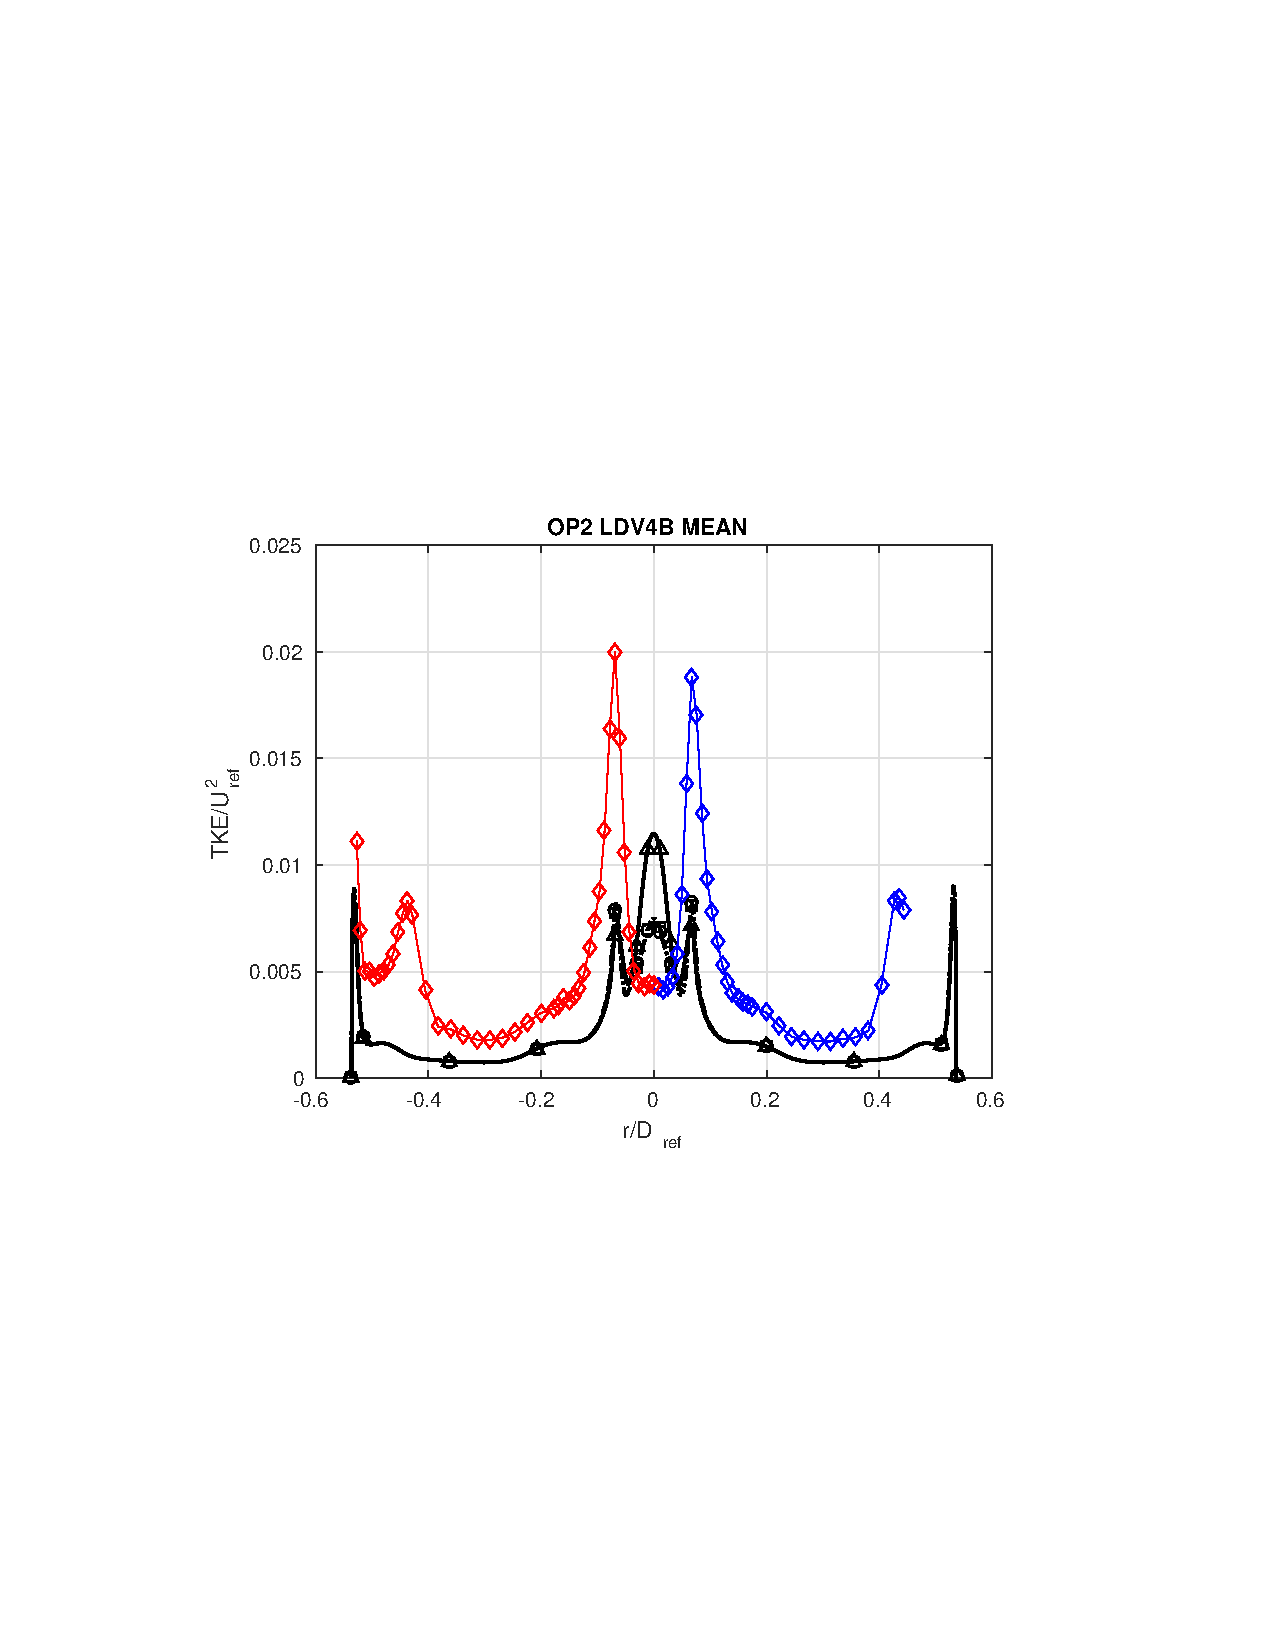
\includegraphics[clip=true, trim= 3.0cm 8.0cm 4.0cm 8.0cm,width=0.98\linewidth]{./figures/bulbt/4BY0/14m/multi_plan4BY0_BulbT_op2_Tke_X}} \\
     \subfigure[]{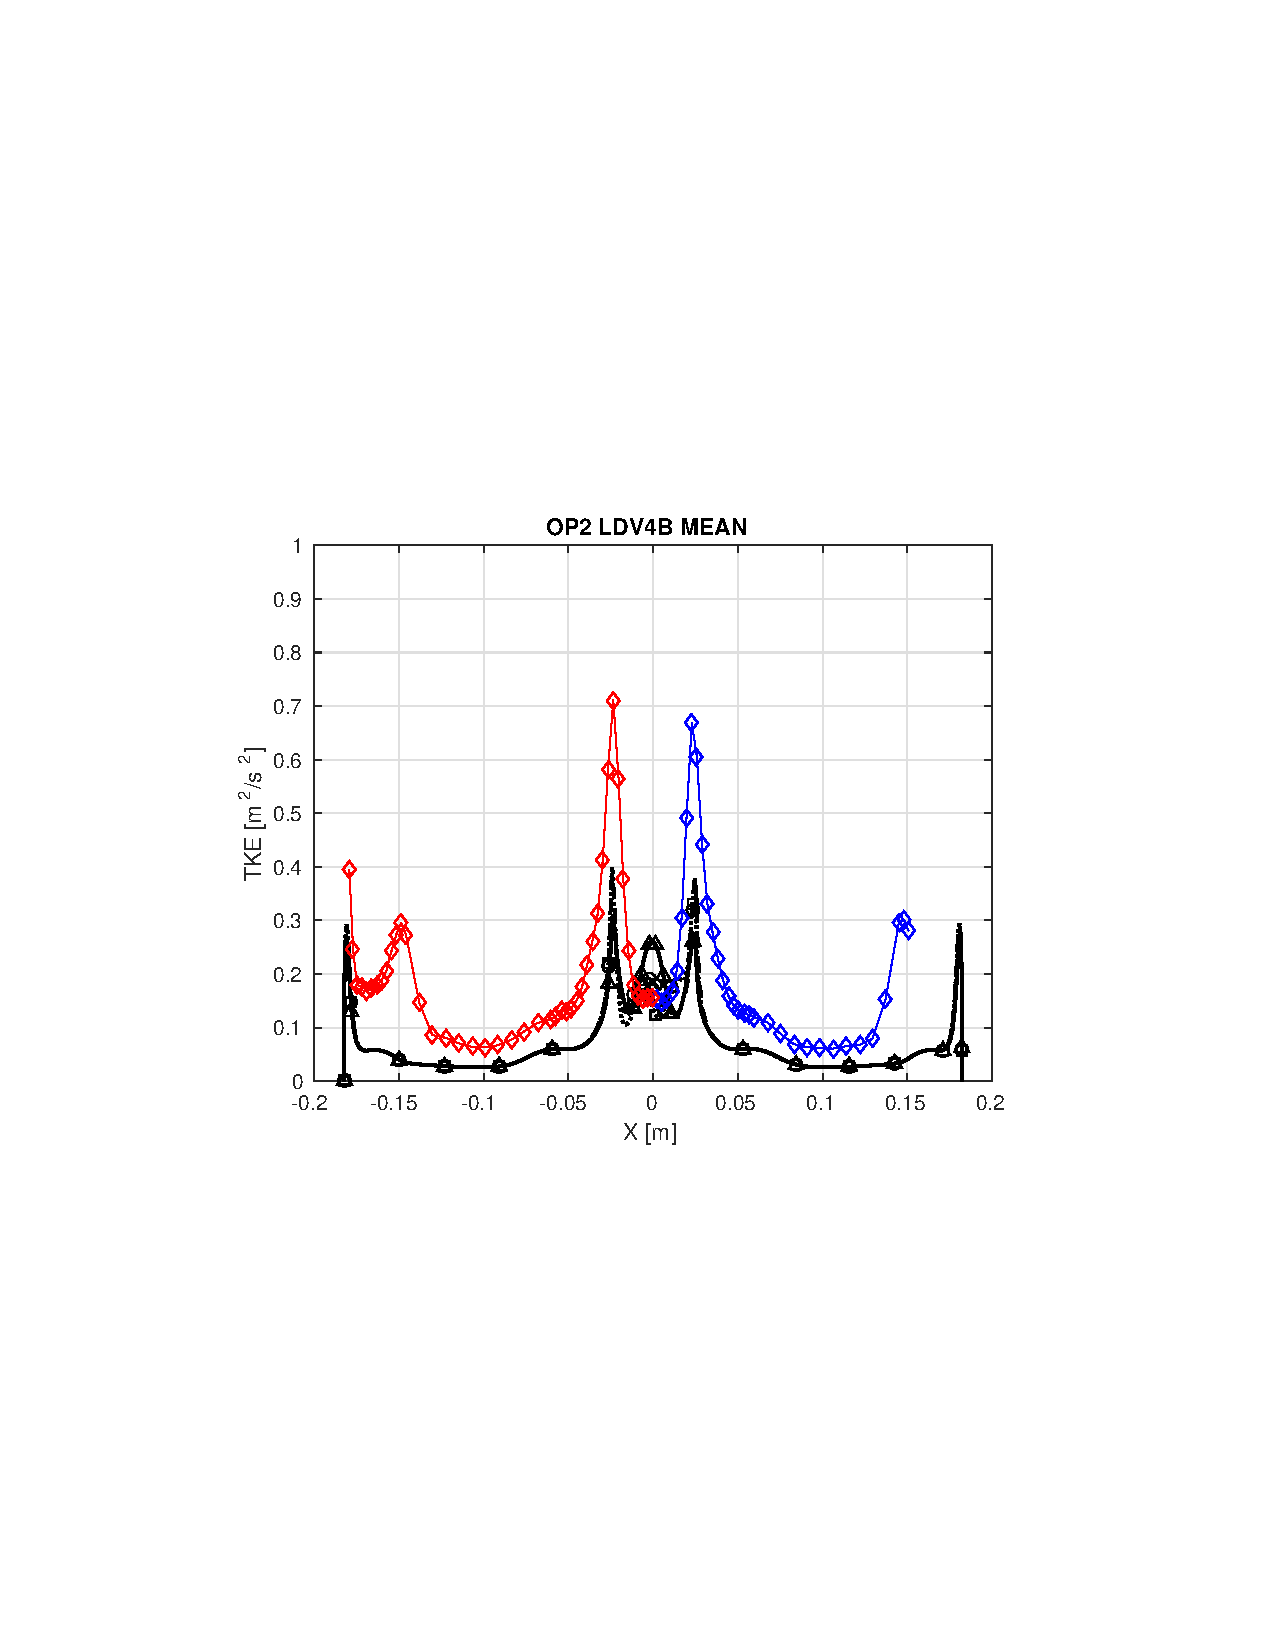
\includegraphics[clip=true, trim= 3.0cm 8.0cm 4.0cm 8.0cm,width=0.98\linewidth]{./figures/bulbt/4BY0/50m/multi_plan4BY0_BulbT_op2_Tke_X}}        
     \caption{TKE profiles at plane 4BY0 on (a)3M (b)14M (c)50M grid.  (MUSCL: \mline; EDDY: \eline; EDDY-P: \epline; EXP TKE Az0: \bluediam; EXP TKE Az180: \reddiam.)}
     \label{tke} 
%     \end{minipage}          
\end{figure}
%%%%%%%%%%%%%%%%%%%%%%%%%%%%%%%%%%%%%%%%%%%%%%%%%%%%%%%%%%%%%%%%
\begin{figure}[t]  
\centering
%\begin{minipage}{.99\textwidth}
\centering
     \subfigure[]{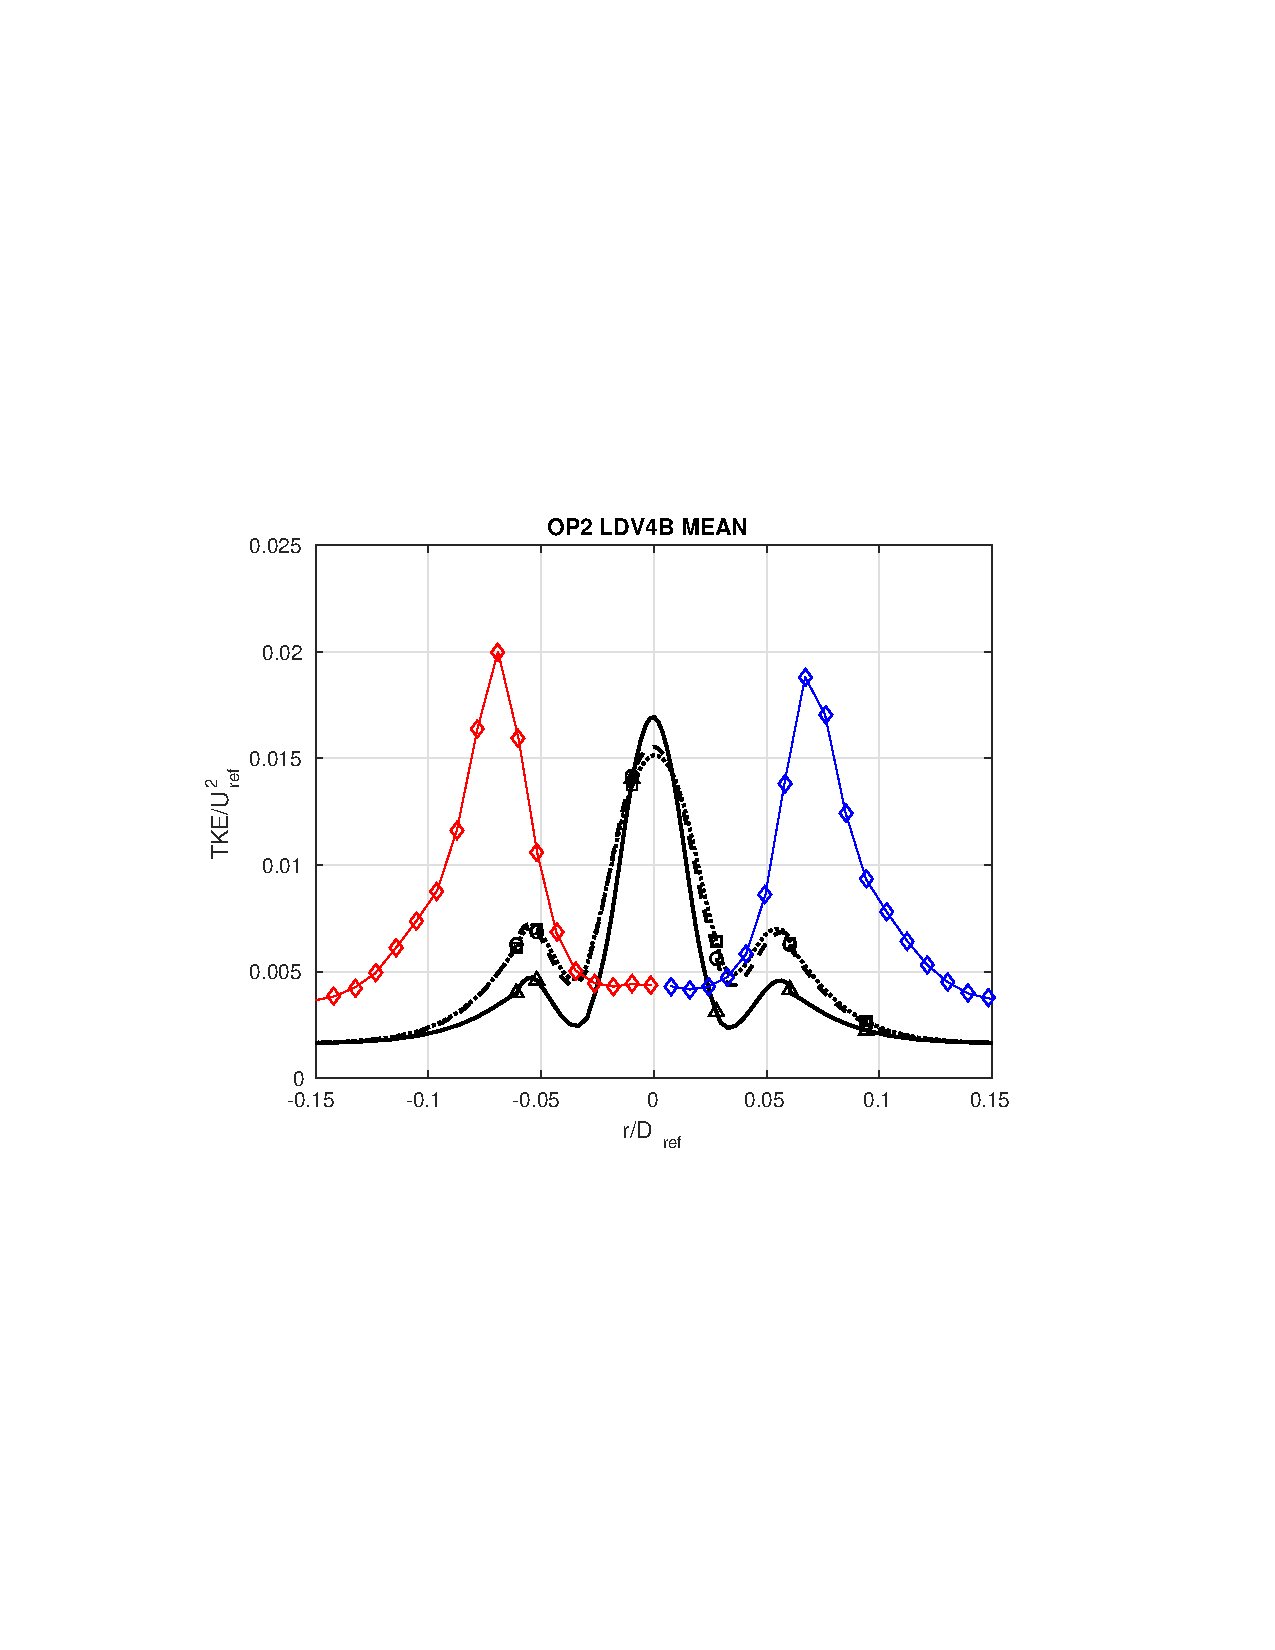
\includegraphics[clip=true, trim= 3.0cm 8.0cm 4.0cm 8.0cm,width=0.98\linewidth]{./figures/bulbt/4BY0/3m/zoom_multi_plan4BY0_BulbT_op2_Tke_X}} \\             
     \subfigure[]{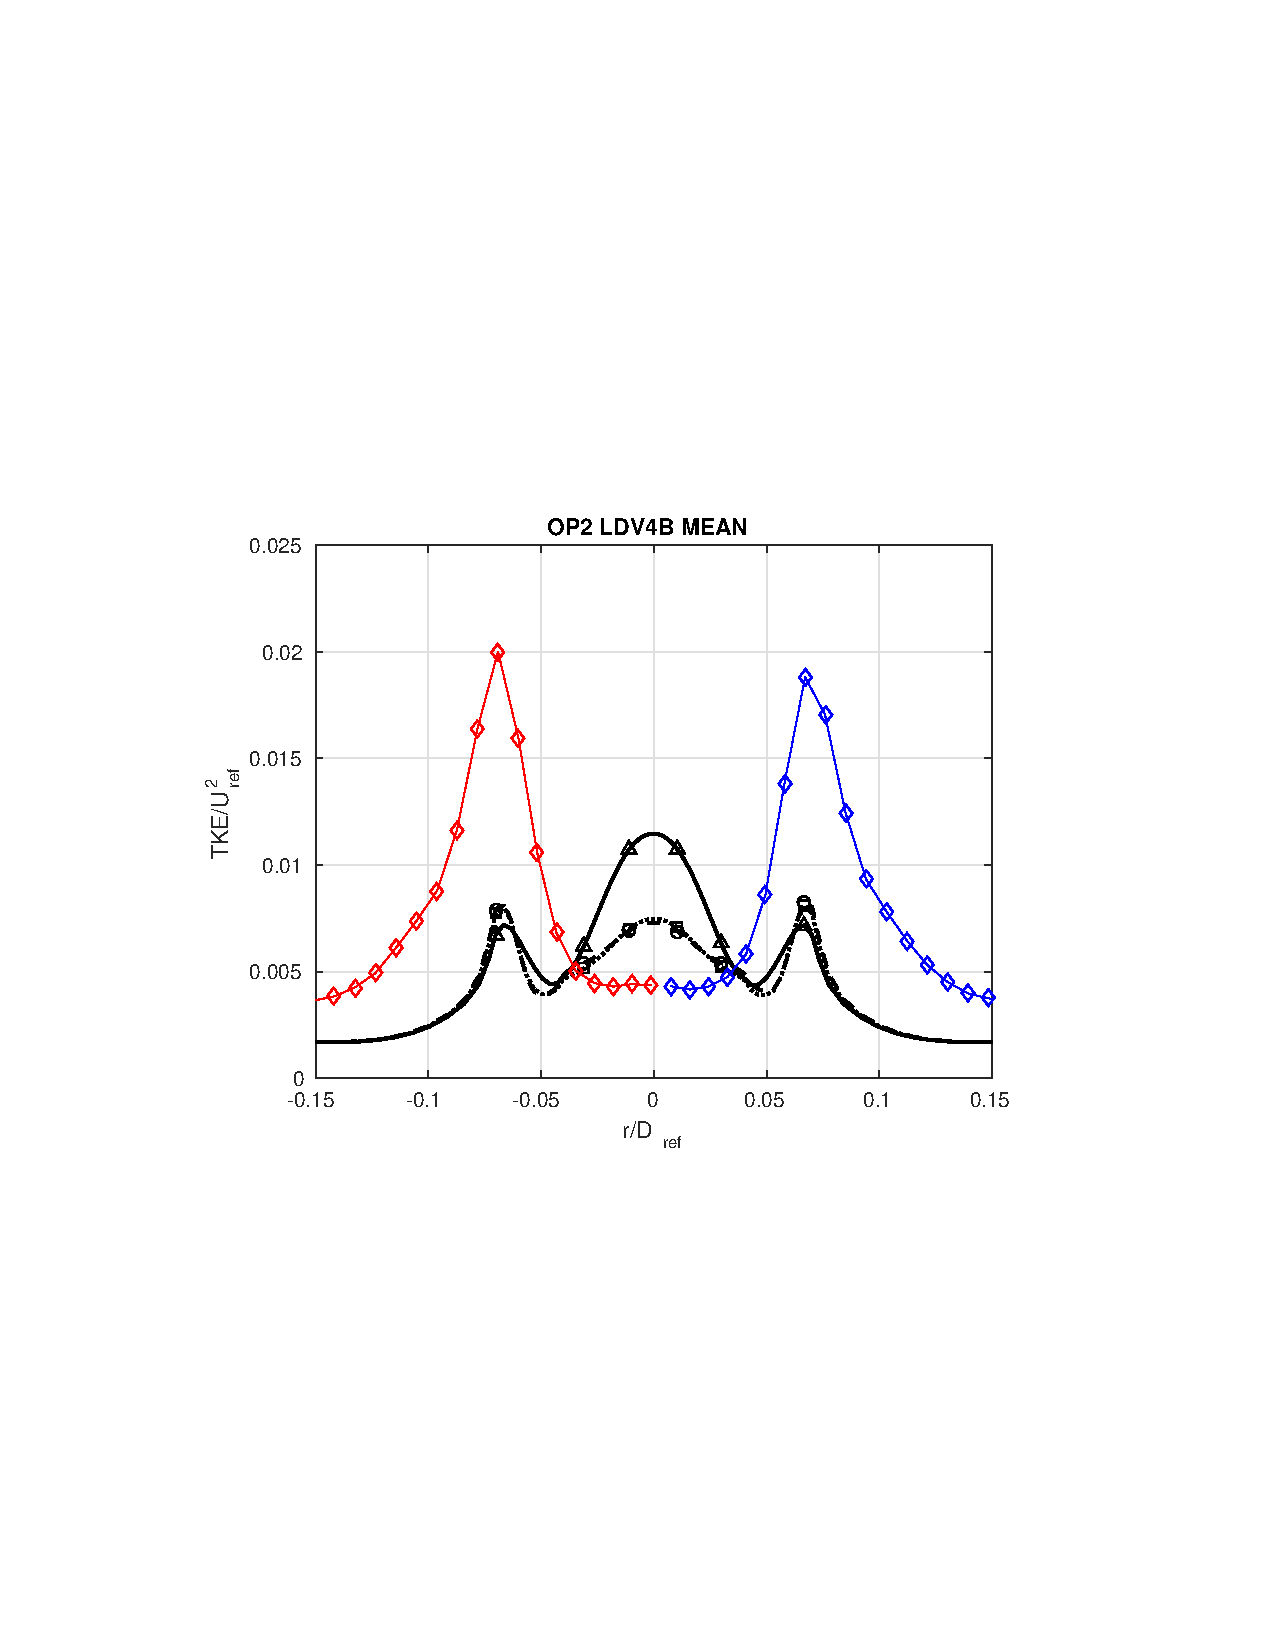
\includegraphics[clip=true, trim= 3.0cm 8.0cm 4.0cm 8.0cm,width=0.98\linewidth]{./figures/bulbt/4BY0/14m/zoom_multi_plan4BY0_BulbT_op2_Tke_X}} \\
     \subfigure[]{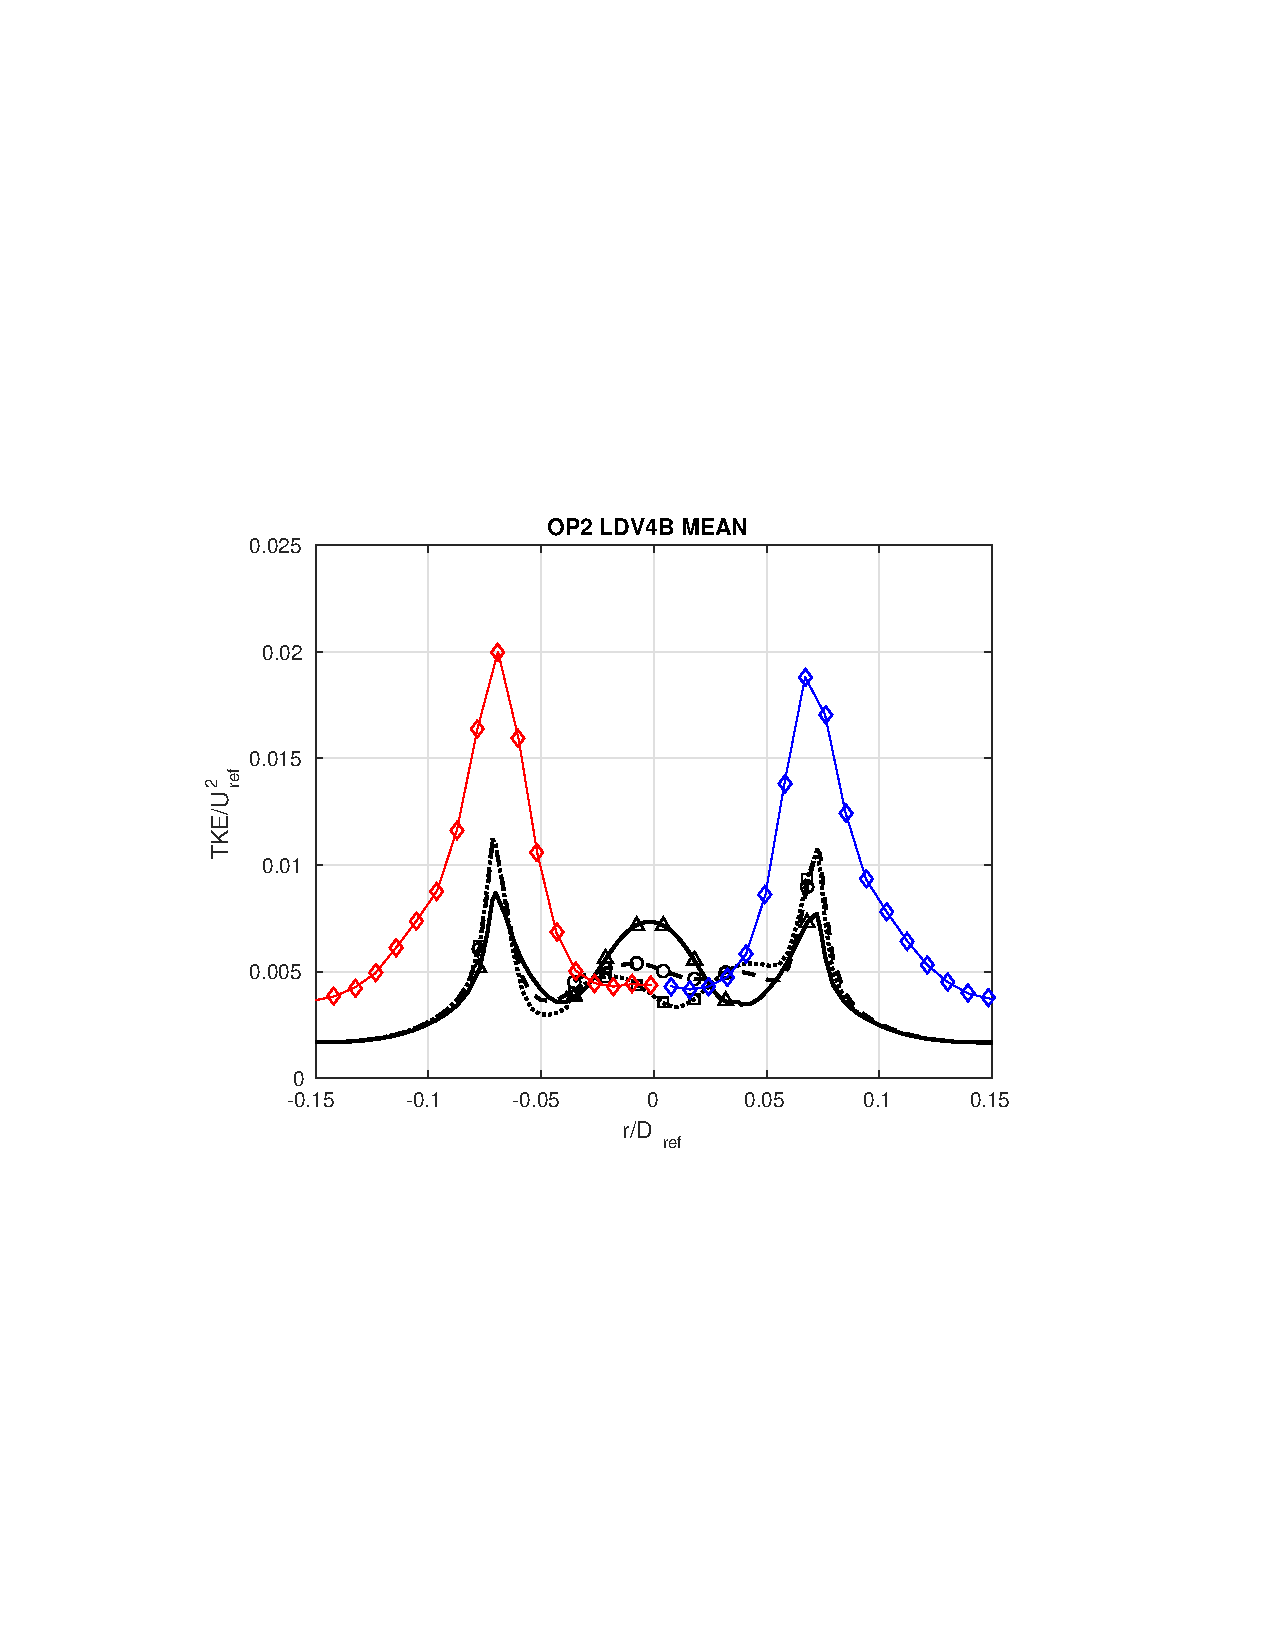
\includegraphics[clip=true, trim= 3.0cm 8.0cm 4.0cm 8.0cm,width=0.98\linewidth]{./figures/bulbt/4BY0/50m/zoom_multi_plan4BY0_BulbT_op2_Tke_X}}       
     \caption{Zoom-in view of TKE profiles at plane 4BY0 on (a)3M (b)14M (c)50M grid. (MUSCL: \mline; EDDY: \eline; EDDY-P: \epline; EXP TKE Az0: \bluediam; EXP TKE Az180: \reddiam.)}
     \label{ztke} 
%     \end{minipage}          
\end{figure}
%%%%%%%%%%%%%%%%%%%%%%%%%%%%%%%%%%%%%%%%%%%%%%%%%%%%%%%%%%%%%%%%
%%%%%%%%%%%%%%%%%%%%%%%%%%%%%%%%%%%%%%%%%%%%%%%%%%%%%%%%%%%%%%%%
%%%%%%%%%%%%%%%%%%%%%%%%%%%%%%%%%%%%%%%%%%%%%%%%%%%%%%%%%%%%%%%%
%%%%%%%%%%%%%%%%%%%%%%%%%%%%%%%%%%%%%%%%%%%%%%%%%%%%%%%%%%%%%%%%
\begin{figure}[t]  
\centering
%\begin{minipage}{.99\textwidth}
\centering
     \subfigure[]{\includegraphics[clip=true, trim= 1.25cm 1.25cm 3.25cm 3.25cm,width=0.98\linewidth]{./figures/bulbt/P/3m}} \\             
     \subfigure[]{\includegraphics[clip=true, trim= 1.25cm 1.25cm 3.25cm 3.25cm,width=0.98\linewidth]{./figures/bulbt/P/14m}} \\
     \subfigure[]{\includegraphics[clip=true, trim= 1.25cm 1.25cm 3.25cm 3.25cm,width=0.98\linewidth]{./figures/bulbt/P/50m}}     
     \caption{Pressure profiles at plane 4BY0 on (a)3M (b)14M (c)50M grid.}
     \label{p}     
%     \end{minipage}          
\end{figure}
%%%%%%%%%%%%%%%%%%%%%%%%%%%%%%%%%%%%%%%%%%%%%%%%%%%%%%%%%%%%%%%%
%%%%%%%%%%%%%%%%%%%%%%%%%%%%%%%%%%%%%%%%%%%%%%%%%%%%%%%%%%%%%%%%
%%%%%%%%%%%%%%%%%%%%%%%%%%%%%%%%%%%%%%%%%%%%%%%%%%%%%%%%%%%%%%%%
%%%%%%%%%%%%%%%%%%%%%%%%%%%%%%%%%%%%%%%%%%%%%%%%%%%%%%%%%%%%%%%%
\begin{figure}[t]  
\centering
%\begin{minipage}{.99\textwidth}
\centering
     \subfigure[]{\includegraphics[clip=true, trim= 1.25cm 1.25cm 3.25cm 3.25cm,width=0.98\linewidth]{./figures/bulbt/4by0vo/3m}} \\            
     \subfigure[]{\includegraphics[clip=true, trim= 1.25cm 1.25cm 3.25cm 3.25cm,width=0.98\linewidth]{./figures/bulbt/4by0vo/14m}} \\
     \subfigure[]{\includegraphics[clip=true, trim= 1.25cm 1.25cm 3.25cm 3.25cm,width=0.98\linewidth]{./figures/bulbt/4by0vo/50m}}        
     \caption{Vorticity magnitude at plane 4BY0 on (a)3M (b)14M (c)50M grid. (MUSCL: \mline; EDDY: \eline; EDDY-P: \epline; EXP: \exact.)}
     \label{vo} 
%     \end{minipage}          
\end{figure}
%%%%%%%%%%%%%%%%%%%%%%%%%%%%%%%%%%%%%%%%%%%%%%%%%%%%%%%%%%%%%%%%
%\FloatBarrier
\begin{table}[t]
\caption{Relative $L^{2}$ norms of difference for pressure profiles.}
\begin{center}
\label{table2}
\begin{tabular}{c l l l}
\hline
Scheme & 3M     & 14M    & 50M    \\ 
\hline
MUSCL  & 0.2872 & 0.0953 & 0.0458 \\ 
EDDY   & 0.2105 & 0.0776 & 0.0166 \\ 
EDDY-P & 0.0750 & 0.0743 & 0.0000 \\
\hline 
\end{tabular}
\end{center}
\end{table}
%%%%%%%%%%%%%%%%%%%%%%%%%%%%%%%%%%%%%%%%%%%%%%%%%%%%%%%%%%%%%%%%












































%%%%%%%%%%%%%%%%%%%%%%%%%%%%%%%%%%%%%%%%%%%%%%%%%%%%%%%%%%%%%%%%%%
%%\begin{figure}[!htb]  
%%\centering
%%\begin{minipage}{.99\textwidth}
%%\centering
%%     \subfigure[]{\includegraphics[clip=true, trim= 3.0cm 8.0cm 4.0cm 8.0cm,width=0.98\linewidth]{./figures/bulbt/4BY0/3m/multi_plan4BY0_BulbT_op2_uncert_X}} \\             
%%     \subfigure[]{\includegraphics[clip=true, trim= 3.0cm 8.0cm 4.0cm 8.0cm,width=0.98\linewidth]{./figures/bulbt/4BY0/14m/multi_plan4BY0_BulbT_op2_uncert_X}} \\
%%     \subfigure[]{\includegraphics[clip=true, trim= 3.0cm 8.0cm 4.0cm 8.0cm,width=0.98\linewidth]{./figures/bulbt/4BY0/50m/multi_plan4BY0_BulbT_op2_uncert_X}}  \\       
%%     \caption{Velocity profiles at plane 4BY0 on (a)3M (b)14M (c)50M grid. (MUSCL: \mline; EDDY: \eline; EDDY-P: \epline; EXP Cz Az0: \bluediam; EXP Cz Az180: \reddiam; EXP Cy Az0: \bluecrx; EXP Cy Az180: \redcrx.)}
%%     \label{u} 
%%     \end{minipage}          
%%\end{figure}
%%%%%%%%%%%%%%%%%%%%%%%%%%%%%%%%%%%%%%%%%%%%%%%%%%%%%%%%%%%%%%%%%%
%%\begin{figure}[!htb]  
%%\centering
%%\begin{minipage}{.99\textwidth}
%%\centering
%%     \subfigure[]{\includegraphics[clip=true, trim= 3.0cm 8.0cm 4.0cm 8.0cm,width=0.98\linewidth]{./figures/bulbt/4BY0/3m/zoom_multi_plan4BY0_BulbT_op2_uncert_X}} \\             
%%     \subfigure[]{\includegraphics[clip=true, trim= 3.0cm 8.0cm 4.0cm 8.0cm,width=0.98\linewidth]{./figures/bulbt/4BY0/14m/zoom_multi_plan4BY0_BulbT_op2_uncert_X}} \\
%%     \subfigure[]{\includegraphics[clip=true, trim= 3.0cm 8.0cm 4.0cm 8.0cm,width=0.98\linewidth]{./figures/bulbt/4BY0/50m/zoom_multi_plan4BY0_BulbT_op2_uncert_X}} \\        
%%     \caption{Zoom-in view of velocity profiles at plane 4BY0 on (a)3M (b)14M (c)50M grid. (MUSCL: \mline; EDDY: \eline; EDDY-P: \epline; EXP Cz Az0: \bluediam; EXP Cz Az180: \reddiam; EXP Cy Az0: \bluecrx; EXP Cy Az180: \redcrx.)}
%%     \label{zu} 
%%     \end{minipage}          
%%\end{figure}
%%%%%%%%%%%%%%%%%%%%%%%%%%%%%%%%%%%%%%%%%%%%%%%%%%%%%%%%%%%%%%%%%%
%%%%%%%%%%%%%%%%%%%%%%
%\begin{figure}[!htb]  
%\centering
%\begin{minipage}{.99\textwidth}
%     \subfigure[]{\includegraphics[clip=true, trim= 3.0cm 8.0cm 4.0cm 8.0cm,width=0.32\linewidth]{./figures/bulbt/4BY0/3m/multi_plan4BY0_BulbT_op2_uncert_X}}              
%     \subfigure[]{\includegraphics[clip=true, trim= 3.0cm 8.0cm 4.0cm 8.0cm,width=0.32\linewidth]{./figures/bulbt/4BY0/14m/multi_plan4BY0_BulbT_op2_uncert_X}} 
%     \subfigure[]{\includegraphics[clip=true, trim= 3.0cm 8.0cm 4.0cm 8.0cm,width=0.32\linewidth]{./figures/bulbt/4BY0/50m/multi_plan4BY0_BulbT_op2_uncert_X}}         
%     \caption{Velocity profiles at plane 4BY0 on (a)3M (b)14M (c)50M grid. (MUSCL: \mline; EDDY: \eline; EDDY-P: \epline; EXP Cz Az0: \bluediam; EXP Cz Az180: \reddiam; EXP Cy Az0: \bluecrx; EXP Cy Az180: \redcrx.)}
%     \label{u} 
%     \end{minipage}          
%\end{figure}
%%%%%%%%%%%%%%%%%%%%%%%%%%%%%%%%%%%%%%%%%%%%%%%%%%%%%%%%%%%%%%%%%
%\begin{figure}[!htb]  
%\centering
%\begin{minipage}{.99\textwidth}
%     \subfigure[]{\includegraphics[clip=true, trim= 3.0cm 8.0cm 4.0cm 8.0cm,width=0.32\linewidth]{./figures/bulbt/4BY0/3m/zoom_multi_plan4BY0_BulbT_op2_uncert_X}}              
%     \subfigure[]{\includegraphics[clip=true, trim= 3.0cm 8.0cm 4.0cm 8.0cm,width=0.32\linewidth]{./figures/bulbt/4BY0/14m/zoom_multi_plan4BY0_BulbT_op2_uncert_X}} 
%     \subfigure[]{\includegraphics[clip=true, trim= 3.0cm 8.0cm 4.0cm 8.0cm,width=0.32\linewidth]{./figures/bulbt/4BY0/50m/zoom_multi_plan4BY0_BulbT_op2_uncert_X}}         
%     \caption{Zoom-in view of velocity profiles at plane 4BY0 on (a)3M (b)14M (c)50M grid. (MUSCL: \mline; EDDY: \eline; EDDY-P: \epline; EXP Cz Az0: \bluediam; EXP Cz Az180: \reddiam; EXP Cy Az0: \bluecrx; EXP Cy Az180: \redcrx.)}
%     \label{zu} 
%     \end{minipage}          
%\end{figure}
%%%%%%%%%%%%%%%%%%%%%%%%%%%%%%%%%%%%%%%%%%%%%%%%%%%%%%%%%%%%%%%%%
%%%%%%%%%%%%%%%%%%%%%%%%%%%%%%%%%%%%%%%%%%%%%%%%%%%%%%%%%%%%%%%%%
%\begin{figure}[!htb]  
%\centering
%\begin{minipage}{.99\textwidth}
%     \subfigure[]{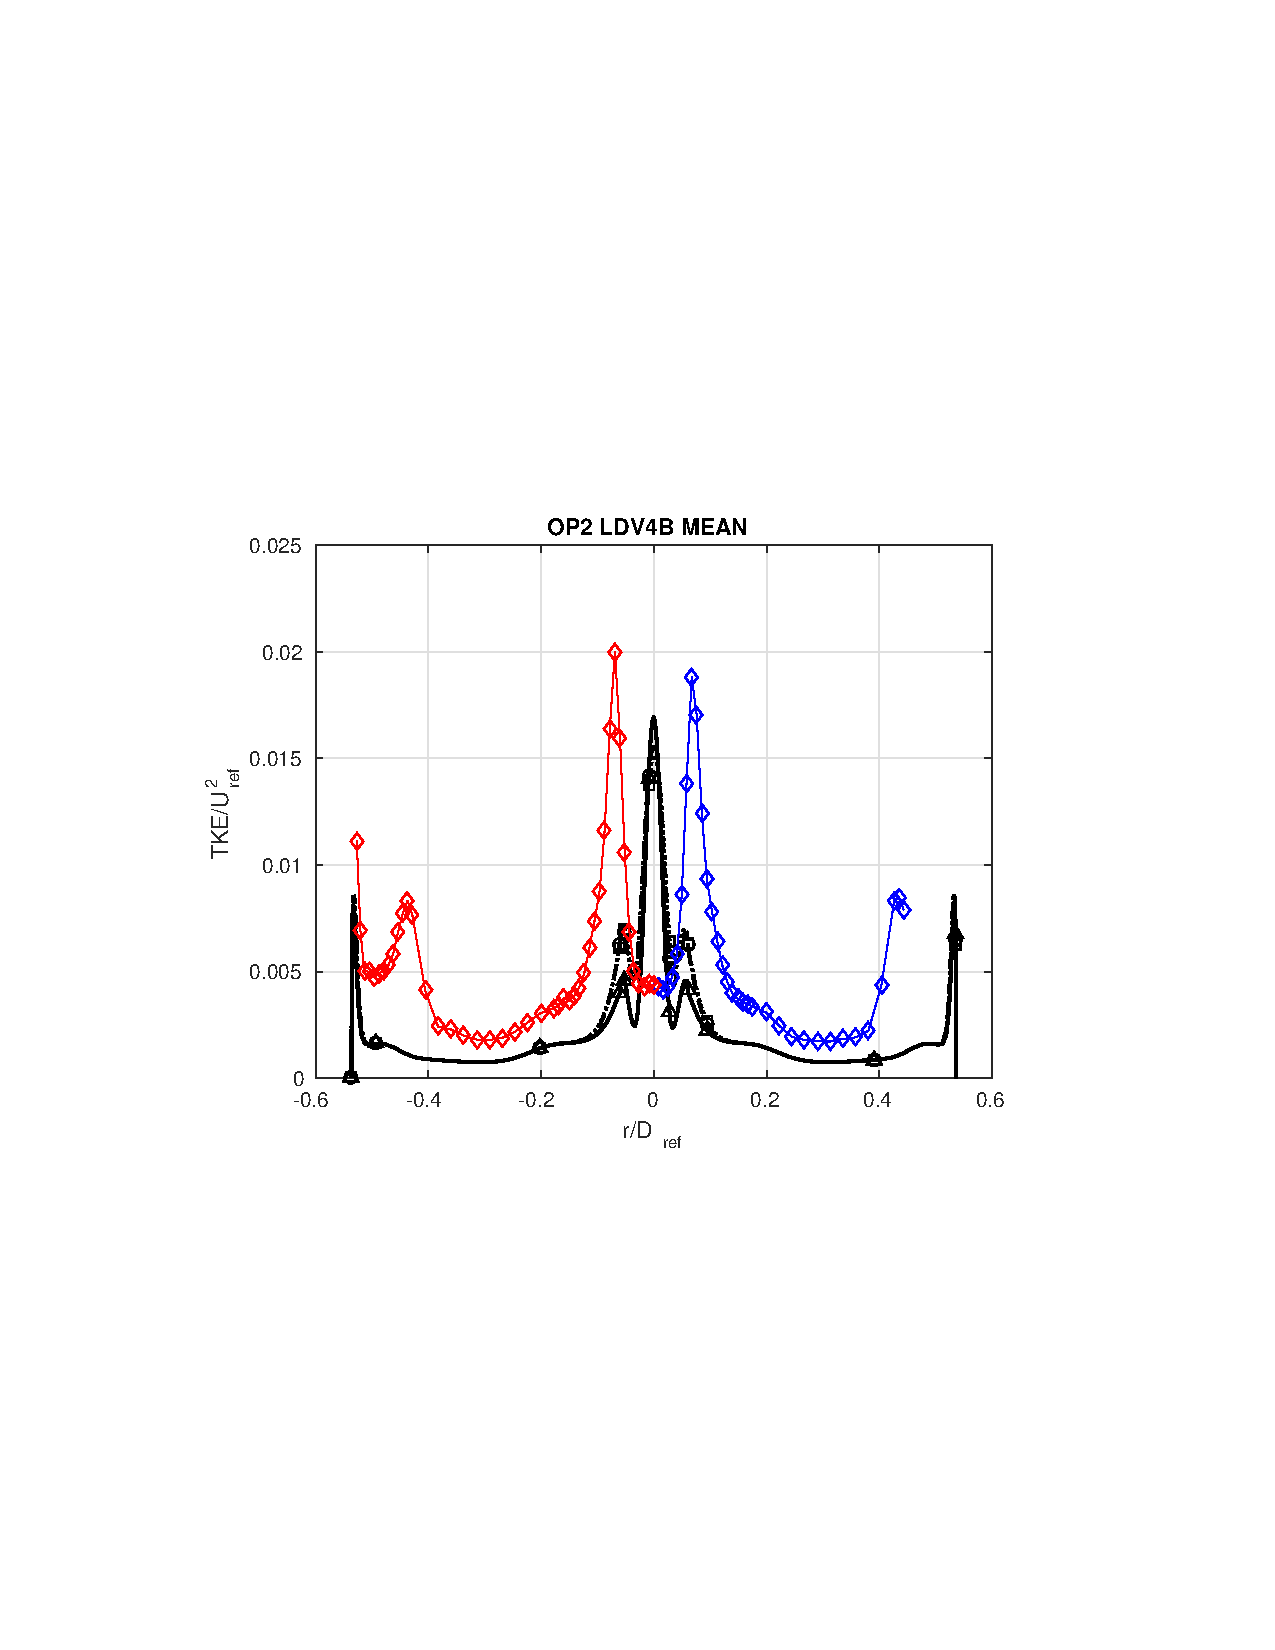
\includegraphics[clip=true, trim= 3.0cm 8.0cm 4.0cm 8.0cm,width=0.32\linewidth]{./figures/bulbt/4BY0/3m/multi_plan4BY0_BulbT_op2_Tke_X}}              
%     \subfigure[]{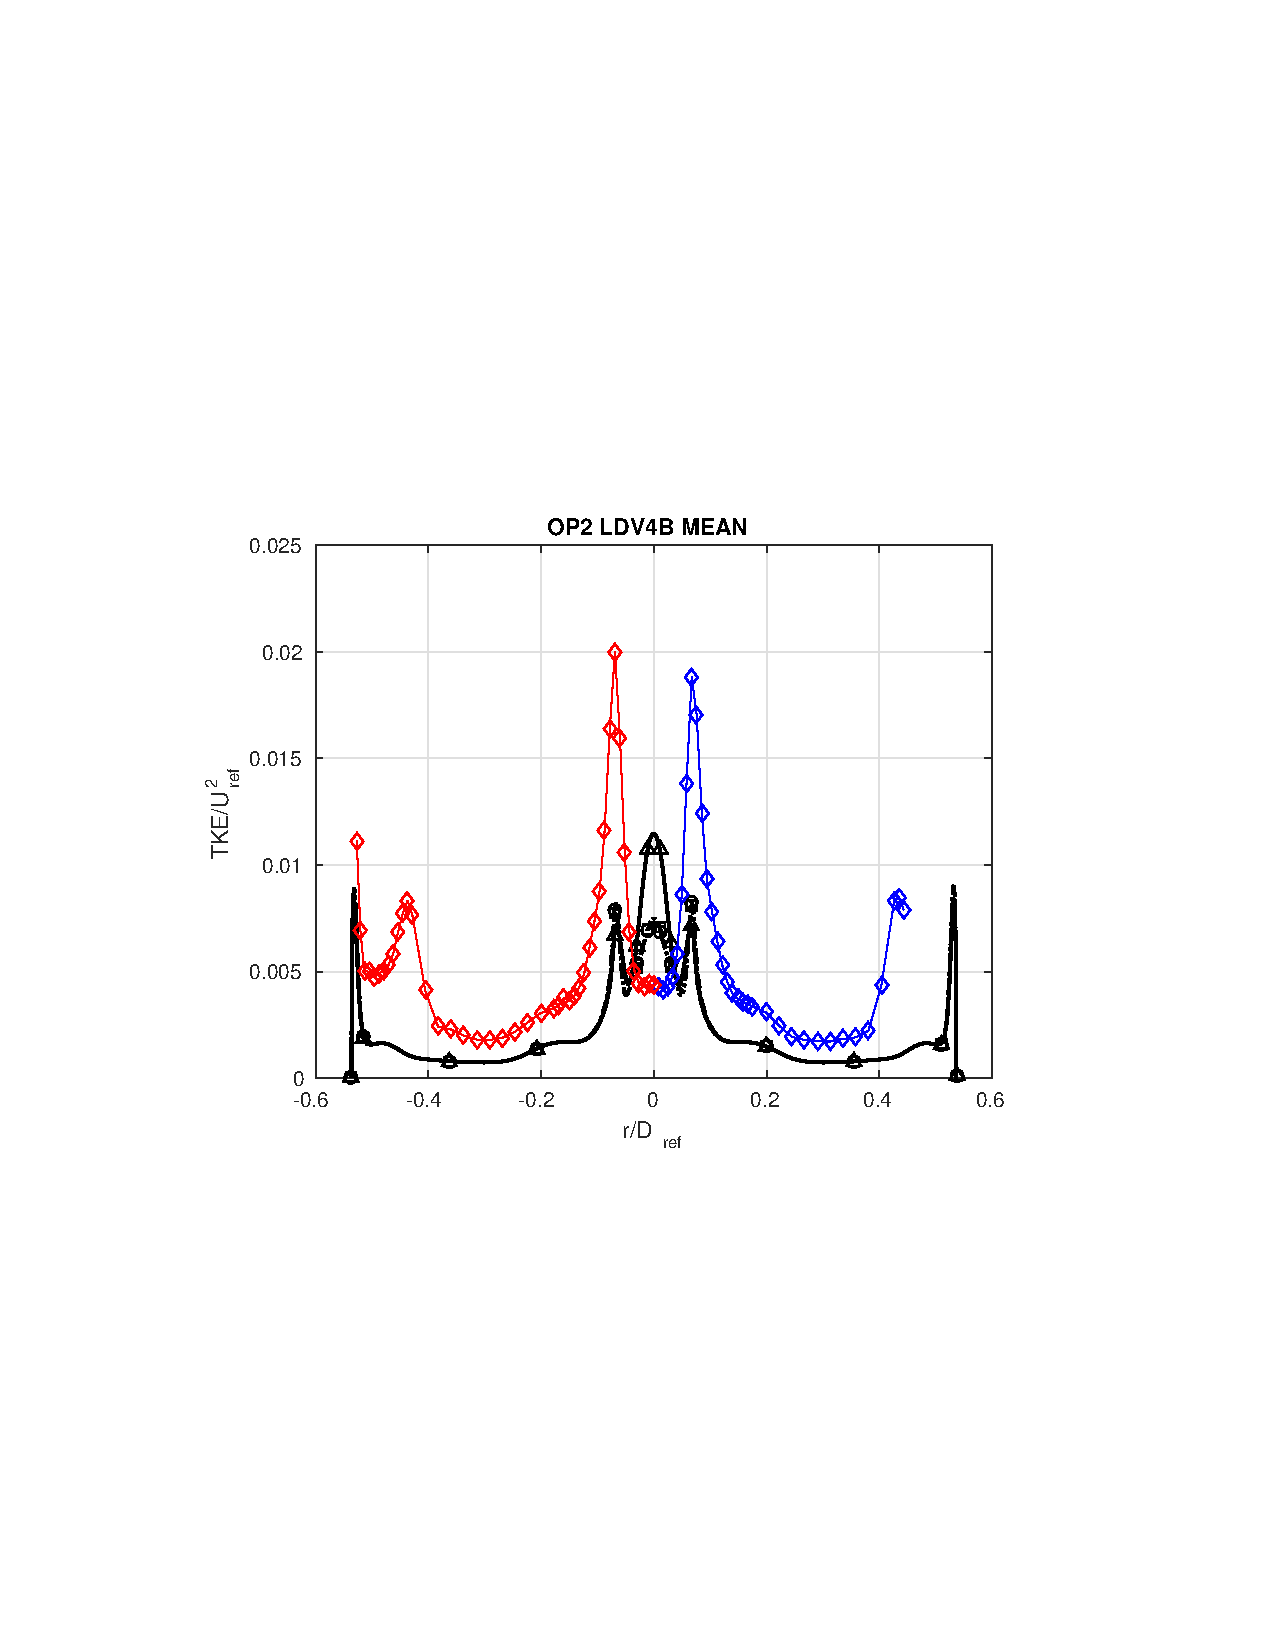
\includegraphics[clip=true, trim= 3.0cm 8.0cm 4.0cm 8.0cm,width=0.32\linewidth]{./figures/bulbt/4BY0/14m/multi_plan4BY0_BulbT_op2_Tke_X}} 
%     \subfigure[]{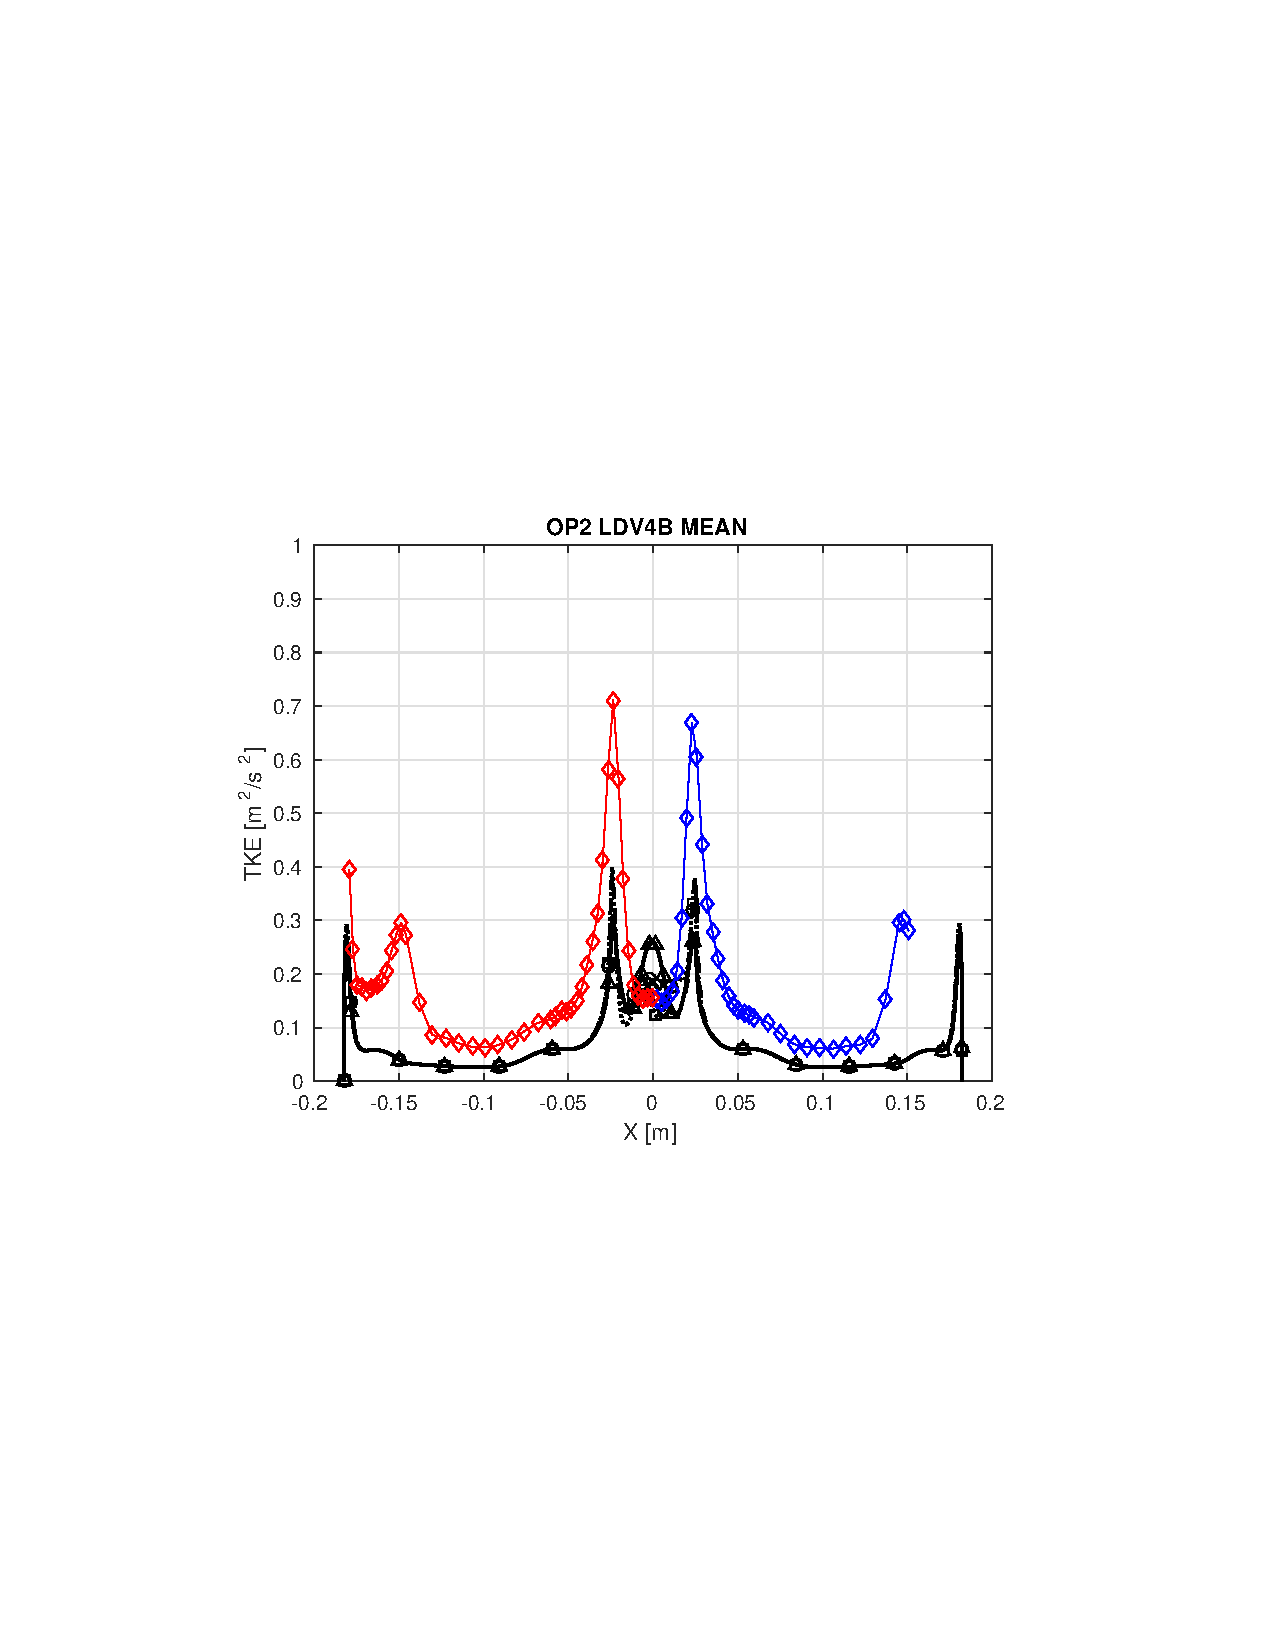
\includegraphics[clip=true, trim= 3.0cm 8.0cm 4.0cm 8.0cm,width=0.32\linewidth]{./figures/bulbt/4BY0/50m/multi_plan4BY0_BulbT_op2_Tke_X}}         
%     \caption{TKE profiles at plane 4BY0 on (a)3M (b)14M (c)50M grid.  (MUSCL: \mline; EDDY: \eline; EDDY-P: \epline; EXP TKE Az0: \bluediam; EXP TKE Az180: \reddiam.)}
%     \label{tke} 
%     \end{minipage}          
%\end{figure}
%%%%%%%%%%%%%%%%%%%%%%%%%%%%%%%%%%%%%%%%%%%%%%%%%%%%%%%%%%%%%%%%%
%\begin{figure}[!htb]  
%\centering
%\begin{minipage}{.99\textwidth}
%     \subfigure[]{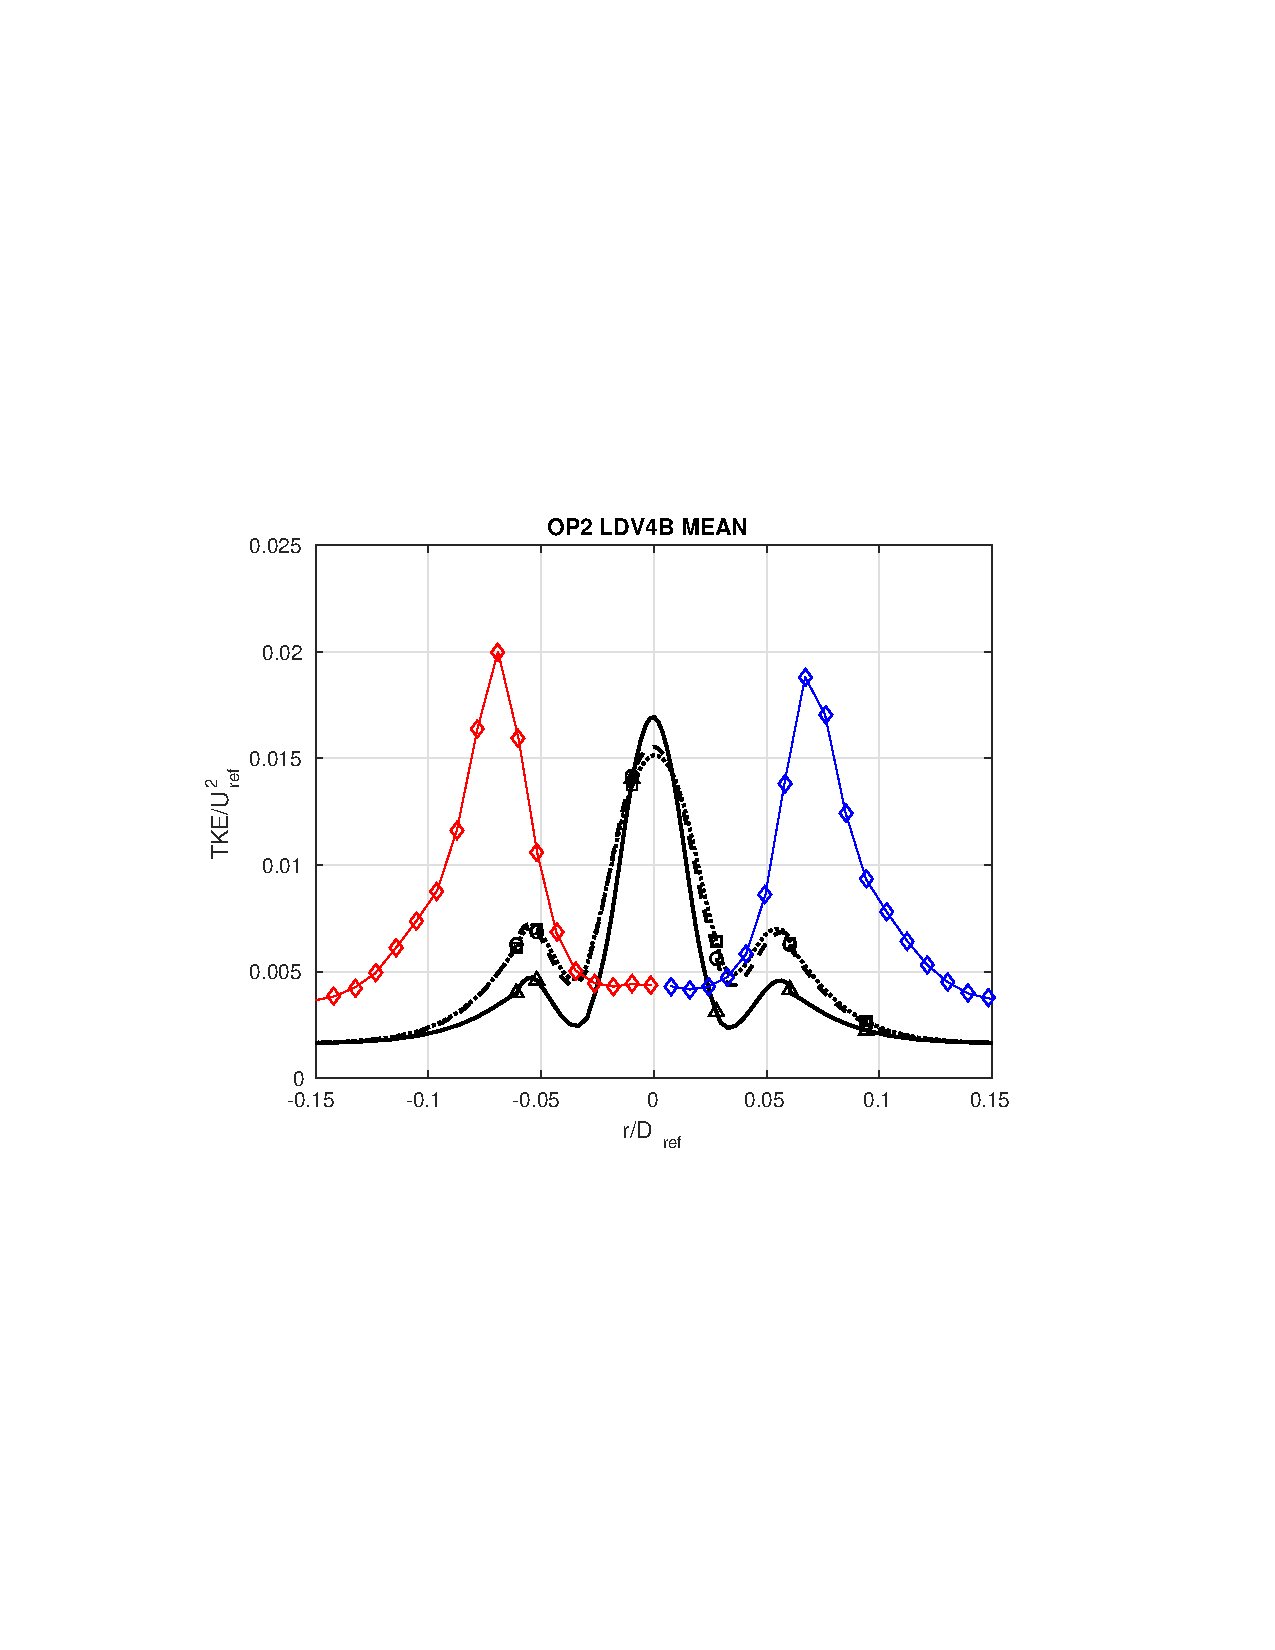
\includegraphics[clip=true, trim= 3.0cm 8.0cm 4.0cm 8.0cm,width=0.32\linewidth]{./figures/bulbt/4BY0/3m/zoom_multi_plan4BY0_BulbT_op2_Tke_X}}              
%     \subfigure[]{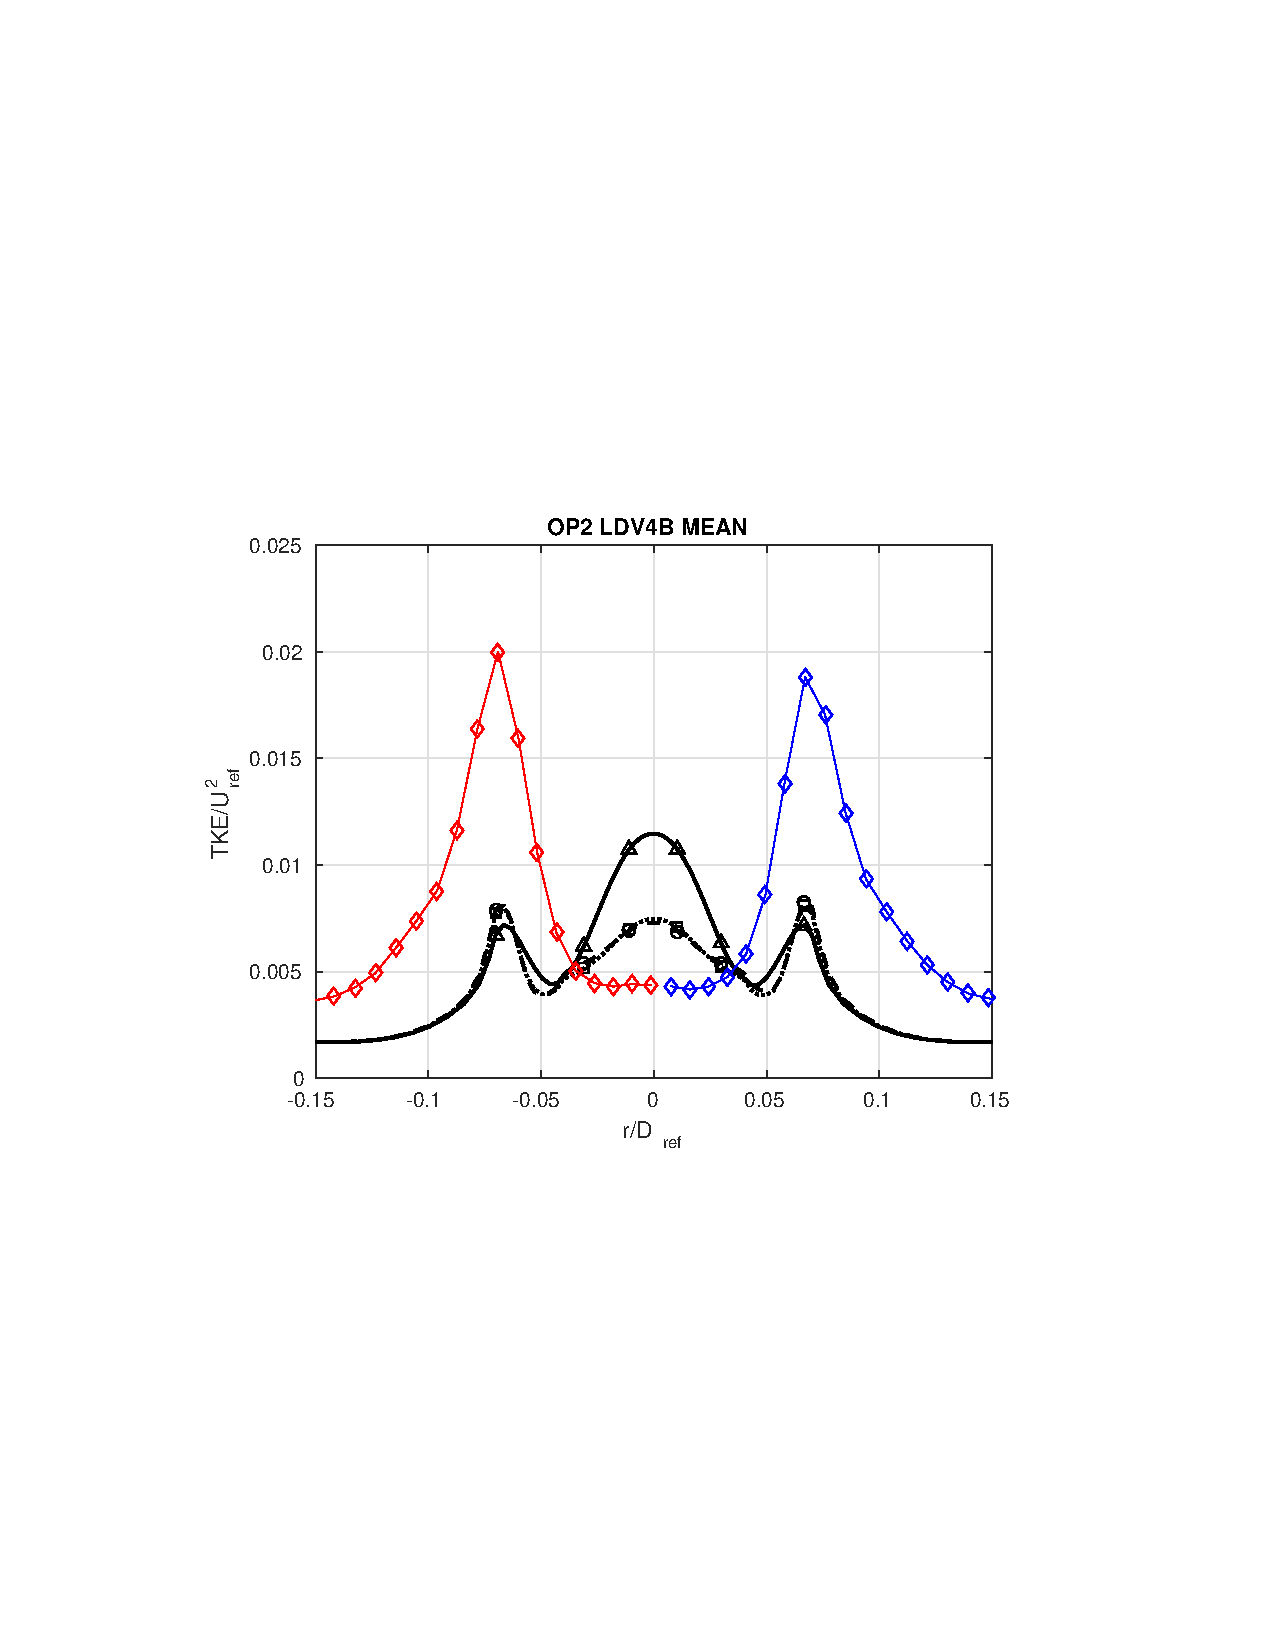
\includegraphics[clip=true, trim= 3.0cm 8.0cm 4.0cm 8.0cm,width=0.32\linewidth]{./figures/bulbt/4BY0/14m/zoom_multi_plan4BY0_BulbT_op2_Tke_X}} 
%     \subfigure[]{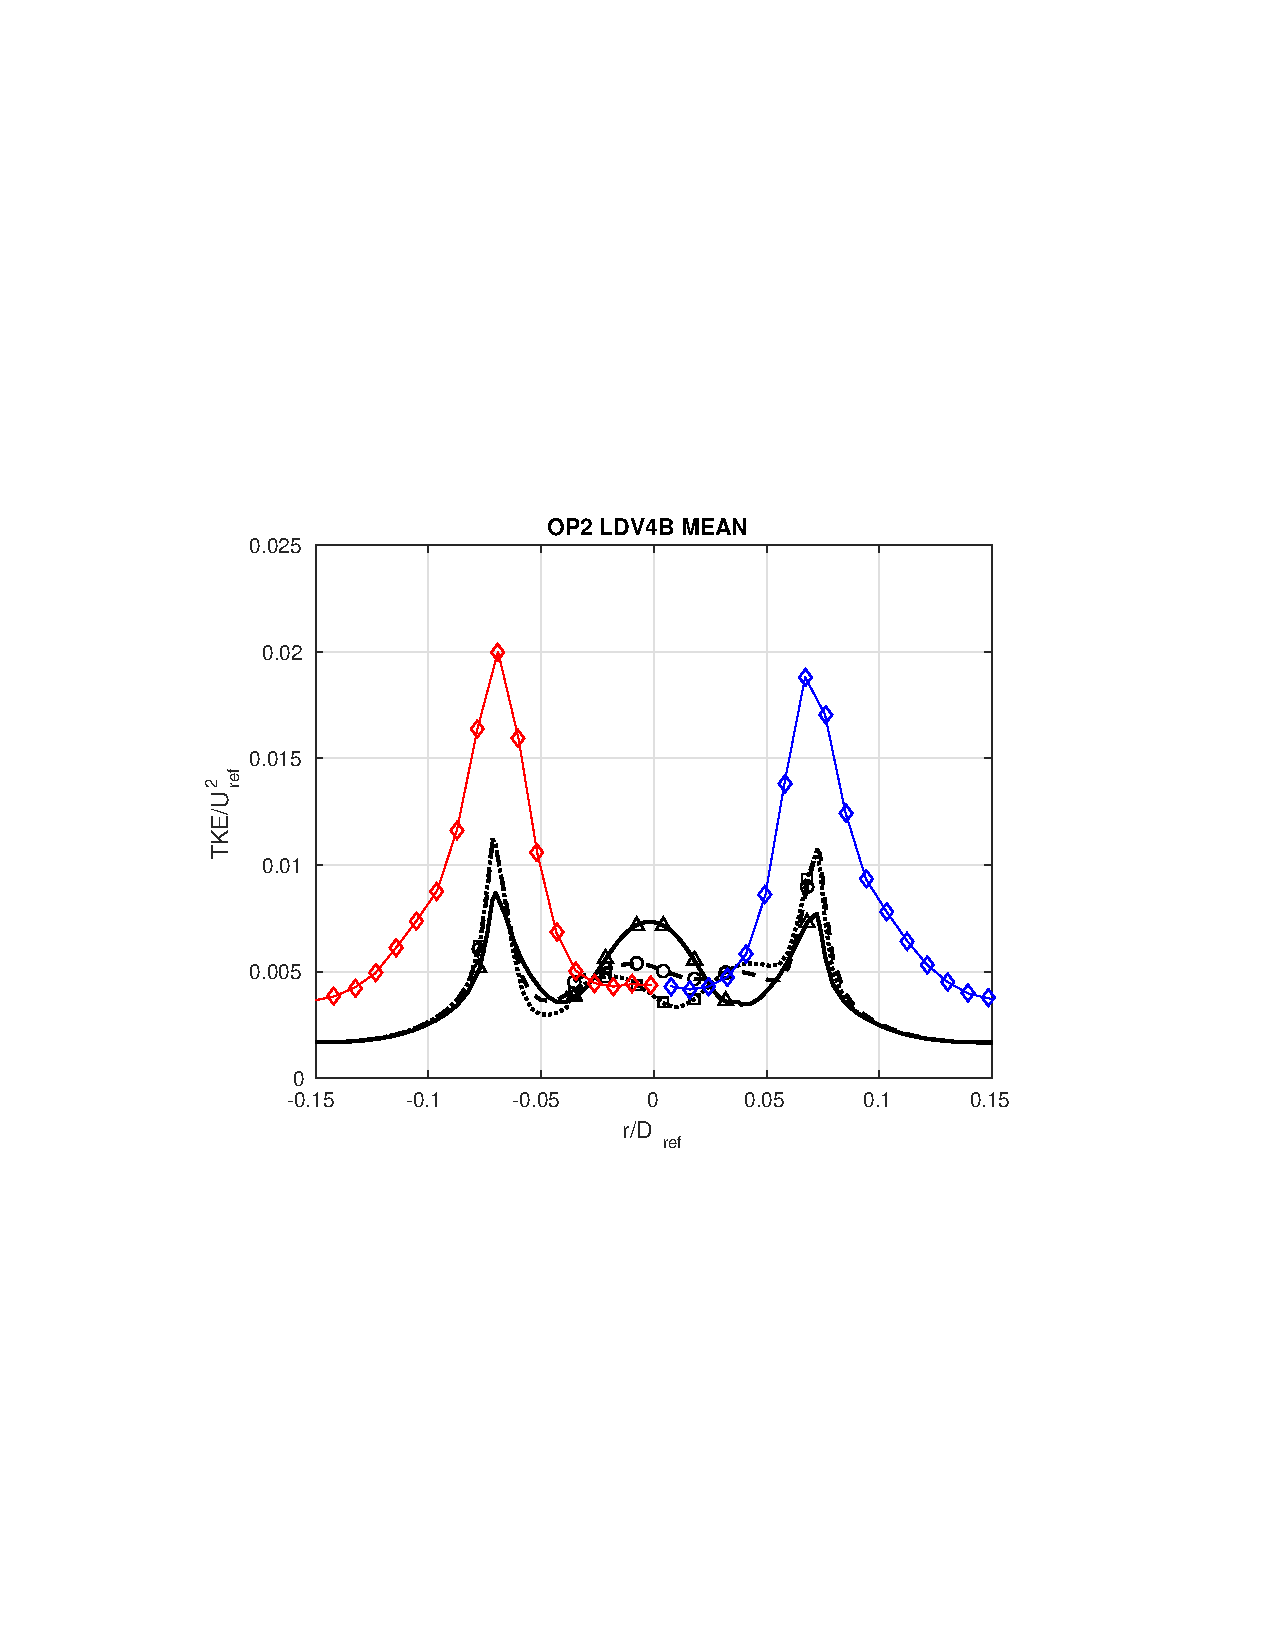
\includegraphics[clip=true, trim= 3.0cm 8.0cm 4.0cm 8.0cm,width=0.32\linewidth]{./figures/bulbt/4BY0/50m/zoom_multi_plan4BY0_BulbT_op2_Tke_X}}         
%     \caption{Zoom-in view of TKE profiles at plane 4BY0 on (a)3M (b)14M (c)50M grid. (MUSCL: \mline; EDDY: \eline; EDDY-P: \epline; EXP TKE Az0: \bluediam; EXP TKE Az180: \reddiam.)}
%     \label{ztke} 
%     \end{minipage}          
%\end{figure}
%%%%%%%%%%%%%%%%%%%%%%%%%%%%%%%%%%%%%%%%%%%%%%%%%%%%%%%%%%%%%%%%%
%%%%%%%%%%%%%%%%%%%%%%%%%%%%%%%%%%%%%%%%%%%%%%%%%%%%%%%%%%%%%%%%%
%%%%%%%%%%%%%%%%%%%%%%%%%%%%%%%%%%%%%%%%%%%%%%%%%%%%%%%%%%%%%%%%%
%%%%%%%%%%%%%%%%%%%%%%%%%%%%%%%%%%%%%%%%%%%%%%%%%%%%%%%%%%%%%%%%%
%\begin{figure}[!htbp]  
%\centering
%\begin{minipage}{.99\textwidth}
%     \subfigure[]{\includegraphics[clip=true, trim= 1.25cm 1.25cm 3.25cm 3.5cm,width=0.32\linewidth]{./figures/bulbt/P/3m2}}              
%     \subfigure[]{\includegraphics[clip=true, trim= 1.25cm 1.25cm 3.25cm 3.5cm,width=0.32\linewidth]{./figures/bulbt/P/14m2}} 
%     \subfigure[]{\includegraphics[clip=true, trim= 1.25cm 1.25cm 3.25cm 3.5cm,width=0.32\linewidth]{./figures/bulbt/P/50m2}}         
%     \caption{Pressure profiles at plane 4BY0 on (a)3M (b)14M (c)50M grid.}
%     \label{p}     
%     \end{minipage}          
%\end{figure}
%%%%%%%%%%%%%%%%%%%%%%%%%%%%%%%%%%%%%%%%%%%%%%%%%%%%%%%%%%%%%%%%%
%%%%%%%%%%%%%%%%%%%%%%%%%%%%%%%%%%%%%%%%%%%%%%%%%%%%%%%%%%%%%%%%%
%\begin{table}[!htbp]
%\centering
%\caption{Relative $L^{2}$ norms of difference for pressure profiles.}
%\label{table2}
%\begin{tabular}{|c|c|c|c|}
%\hline
%            & 3M     & 14M    & 50M    \\ \hline
%MUSCL  & 0.2813 & 0.2049 & 0.0875 \\ \hline
%EDDY   & 0.0895 & 0.0719 & 0.0646 \\ \hline
%EDDY-P & 0.0502 & 0.0182 & 0.0000 \\ \hline
%\end{tabular}
%\end{table}
%%%%%%%%%%%%%%%%%%%%%%%%%%%%%%%%%%%%%%%%%%%%%%%%%%%%%%%%%%%%%%%%%
%%%%%%%%%%%%%%%%%%%%%%%%%%%%%%%%%%%%%%%%%%%%%%%%%%%%%%%%%%%%%%%%%
%\begin{figure}[!htbp]  
%\centering
%\begin{minipage}{.99\textwidth}
%     \subfigure[]{\includegraphics[clip=true, trim= 1.25cm 1.25cm 3.25cm 3.25cm,width=0.32\linewidth]{./figures/bulbt/4by0vo/3m}}              
%     \subfigure[]{\includegraphics[clip=true, trim= 1.25cm 1.25cm 3.25cm 3.25cm,width=0.32\linewidth]{./figures/bulbt/4by0vo/14m}} 
%     \subfigure[]{\includegraphics[clip=true, trim= 1.25cm 1.25cm 3.25cm 3.25cm,width=0.32\linewidth]{./figures/bulbt/4by0vo/50m}}         
%     \caption{Vorticity magnitude at plane 4BY0 on (a)3M (b)14M (c)50M grid. (MUSCL: \mline; EDDY: \eline; EDDY-P: \epline; EXP: \exact.)}
%     \label{vo} 
%     \end{minipage}          
%\end{figure}






%\begin{figure}[!htb]  
%\begin{minipage}{.49\textwidth}
%\centering
%     \includegraphics[clip=true, trim= 0.0cm 0.0cm 0.0cm 0.0cm,width=0.89\linewidth]{./figures/bulbt}                            
%     \caption{Turbine model of BulbT \cite{vuillemard2014experimental}.}
%     \label{bulbt} 
%\end{minipage}
%\begin{minipage}{.49\textwidth}
%     \includegraphics[clip=true, trim= 0.0cm 3.0cm 0.0cm 3.0cm,width=0.89\linewidth]{./figures/bulbt-op}                  
%     \caption{Operating points of BulbT \cite{vuillemard2014experimental}.}
%     \label{bulbt-op}
%\end{minipage}              
%\end{figure}
%%%%%%%%%%%%%%%%%%%%%%%%%%%%%%%%%%%%%%%%%%%%%%%%%%%%%%%%%%%%
%\begin{figure}[!htb]  
%\begin{minipage}{.49\textwidth}
%\centering
%     \includegraphics[clip=true, trim= 1.75cm 6.5cm 1.75cm 0.0cm,width=0.89\linewidth]{./figures/geometry}                            
%     \caption{Geometry of the grid.}
%     \label{grid} 
%\end{minipage}
%\begin{minipage}{.49\textwidth}
%     \includegraphics[clip=true, trim= 0.0cm 0.0cm 0.0cm 1.0cm,width=0.89\linewidth]{./figures/Location4B}                  
%     \caption{Location of 4BY0 \cite{vuillemard2014experimental}.}
%     \label{plane4BY0}
%\end{minipage}              
%\end{figure}
